\documentclass[11pt, a4paper, oneside]{Thesis} % Paper size, default font size and one-sided paper
\usepackage{floatrow}
\floatsetup[table]{capposition=top}
\usepackage{textcomp}
\usepackage{wrapfig}
\usepackage{lscape}
\usepackage{circuitikz}
\usepackage{rotating}
\usepackage{graphicx}
\usepackage{caption}
\usepackage{amsmath}
\usepackage{upgreek}
\usepackage{gensymb}
\usepackage{csquotes}
\usepackage{pdfpages}
\usepackage{lipsum}
\usepackage{notoccite}
\renewcommand{\chapterautorefname}{Chapter} % Forces capital "Chapter"
%\usepackage[open]{bookmark}
\newcommand{\brak}[1]{\left(#1\right)}
% acronyms
\usepackage{acronym}
\usepackage{array}
\newcolumntype{L}{>{\centering\arraybackslash}m{3cm}}

%\usepackage[acronym]{glossaries}
% prints author names as small caps


\makeatletter
\AtBeginDocument{%
  \renewcommand*{\AC@hyperlink}[2]{%
    \begingroup
      \hypersetup{hidelinks}%
      \hyperlink{#1}{#2}%
    \endgroup
  }%
}
\makeatother





%\usepackage{subcaption} %incompatible with subfig
\graphicspath{{Pictures/}} % Specifies the directory where pictures are stored
\usepackage[square, numbers]{natbib} % Use the natbib reference package - read up on this to edit the reference style; if you want text (e.g. Smith et al., 2012) for the in-text references (instead of numbers), remove 'numbers' v

\hypersetup{urlcolor=black, colorlinks=true} % Colors hyperlinks in blue - change to black if annoyingv`
\title{\ttitle} % Defines the thesis title - don't touch this

\begin{document}
\makeatletter
\renewcommand*{\NAT@nmfmt}[1]{\textsc{#1}}
\makeatother

% prints author names as small caps


\frontmatter % Use roman page numbering style (i, ii, iii, iv...) for the pre-content pages

\setstretch{1.6} % Line spacing of 1.6 (double line spacing)

% Define the page headers using the FancyHdr package and set up for one-sided printing
\fancyhead{} % Clears all page headers and footers
\rhead{\thepage} % Sets the right side header to show the page number
\lhead{} % Clears the left side page header

\pagestyle{fancy} % Finally, use the "fancy" page style to implement the FancyHdr headers

\newcommand{\HRule}{\rule{\linewidth}{0.5mm}} % New command to make the lines in the title page

% PDF meta-data
\hypersetup{pdftitle={\ttitle}}
\hypersetup{pdfsubject=\subjectname}
\hypersetup{pdfauthor=\authornames}
\hypersetup{pdfkeywords=\keywordnames}

%----------------------------------------------------------------------------------------
%	TITLE PAGE
%----------------------------------------------------------------------------------------

\begin{titlepage}
\begin{center}

\HRule \\[0.4cm] % Horizontal line
{\huge \bfseries \ttitle}\\[0.4cm] % Thesis title
\HRule \\[1.5cm] % Horizontal line
 
\large \textit{A thesis submitted in fulfilment of the requirements\\ for the degree of \degreename}\\[0.3cm] % University requirement text
\textit{by}\\[0.4cm]
\authornames \\



\vfill
\graphicspath{ {./Figures/} }
\begin{figure}[hb]
  \centering
  
\includegraphics[width=0.35\linewidth]{figs/IITH.png}
\end{figure}

\DEPTNAME\\ % Research group name and department name
\textsc{ \UNIVNAME}\\[1.5cm] % University name
\large \today\\[2cm] % Date


\end{center}

\end{titlepage}

%----------------------------------------------------------------------------------------
%	DECLARATION PAGE
%	Your institution may give you a different text to place here
%----------------------------------------------------------------------------------------

\vspace{20.00mm}

\vfill

\clearpage % Start a new page
%----------------------------------------------------------------------------------------
%	ABSTRACT PAGE
%----------------------------------------------------------------------------------------

%\addtotoc{Abstract} % Add the "Abstract" page entry to the Contents






%----------------------------------------------------------------------------------------
%	Declaration Page
%----------------------------------------------------------------------------------------



%----------------------------------------------------------------------------------------
%	ACKNOWLEDGEMENTS
%----------------------------------------------------------------------------------------
\clearpage % Start a new page
\setstretch{1.3} % Reset the line-spacing to 1.3 for body text (if it has changed)

\clearpage % Start a new page

%----------------------------------------------------------------------------------------
%	LIST OF CONTENTS/FIGURES/TABLES PAGES
%----------------------------------------------------------------------------------------

\pagestyle{fancy} % The page style headers have been "empty" all this time, now use the "fancy" headers as defined before to bring them back

\lhead{\emph{Contents}} % Set the left side page header to "Contents"
\tableofcontents % Write out the Table of Contents


%----------------------------------------------------------------------------------------
%	ABBREVIATIONS
%----------------------------------------------------------------------------------------




\clearpage % Start a new page

%----------------------------------------------------------------------------------------
%	PHYSICAL CONSTANTS/OTHER DEFINITIONS
%----------------------------------------------------------------------------------------
%
% \clearpage % Start a new page

% \lhead{\emph{Physical Constants}} % Set the left side page header to "Physical Constants"

% \listofconstants{lrcl} % Include a list of Physical Constants (a four column table)
% {
% Speed of Light & $c$ & $=$ & $2.997\ 924\ 58\times10^{8}\ \mbox{ms}^{-\mbox{s}}$ (exact)\\
% % Constant Name & Symbol & = & Constant Value (with units) \\
% }

%----------------------------------------------------------------------------------------
%	SYMBOLS
%----------------------------------------------------------------------------------------

\clearpage % Start a new page

\clearpage % Start a new page





\setstretch{1.3} % Return the line spacing back to 1.3
%
\pagestyle{empty} % Page style needs to be empty for this page
%
%----------------------------------------------------------------------------------------
%	THESIS CONTENT - CHAPTERS
%----------------------------------------------------------------------------------------

\mainmatter % Begin numeric (1,2,3...) page numbering

\pagestyle{fancy} % Return the page headers back to the "fancy" style

% Include the chapters of the thesis as separate files from the Chapters folder
% Uncomment the lines as you write the chapters

% Chapter Template

\chapter{Analytical Solution} % Main chapter title

\label{Chapter1}

\lhead{Chapter 1. \emph{Analytical Solution using Fourier Series}} % Change X to a consecutive number; this is for the header on each page - perhaps a shortened title

%----------------------------------------------------------------------------------------
%	SECTION 1
%----------------------------------------------------------------------------------------

\section{Coefficients of complex exponential Fourier series :} 
We know that we can express a periodic function f(t) as the following 
\begin{align*}
&f(t) = \sum\limits_{n=-\infty}^{n=\infty} C_n e^{j n\omega t} \\
&f(t) = .....+C_{-1}e^{-j\omega t} + C_0 + C_1e^{j\omega t}+.....
\end{align*}
where
\begin{itemize}
\item \textbf{Constant Term :} 
\begin{align*}
&\boxed{C_0 = \frac{1}{T}\int\limits_0^T f(t) dt}
\end{align*}
\item \textbf{$C_k$ term :} 
\begin{align*}
&\boxed{C_k = \frac{1}{T}\int\limits_0^Tf(t)e^{-j\omega kt}dt}
\end{align*}
\end{itemize}
\section{Applying this to given question :} 

In the question we are given with a input signal defined as \\
V(t) = $\begin{cases}
A & 0\leq t \leq \alpha T \\
0 & \alpha T \leq t \leq T
\end{cases}$ \\
Here A = 10 , but we are making it to generalize for any value. \\
The differential equation we get is 
\begin{align*}
L\frac{di}{dt} + iR =V(t)
\end{align*}
The idea we use here is , We write the V(t) in the RHS as sum of complex exponentials and solve the differential equation for individual complex exponential function and add up all the solutions we get to get the current i(t) (Using superposition principle).\\
Let 
\begin{align*}
V(t) = \sum\limits_{n=-\infty}^{n=\infty} C_n e^{j n\omega t}
\end{align*}
Where $\omega = \frac{2\pi}{T}$ \\
Now let us find the coefficients.
\begin{itemize}
\item \textbf{Constant term :} 
\begin{align*}
C_0 &= \frac{1}{T}\int\limits_0^T V(t) dt \\ 
& = \frac{1}{T} \int\limits_0^{\alpha T}A dt + \int\limits_{\alpha T}^T0dt \\
& = \frac{1}{T} [At]_0^{\alpha T} + 0 \\
& = \frac{1}{T} (A \alpha T ) \\
& = A \alpha \\
&\boxed{C_0 = A\alpha}
\end{align*}
\item \textbf{$C_1,C_2,...,C_k$ terms :} 
\begin{align*}
C_k &= \frac{1}{T}\int\limits_0^Tf(t)e^{-j\omega kt}dt \\ 
& = \frac{1}{T} ( \int\limits_0^{\alpha T} A e^{-j\omega kt}dt + \int\limits_{\alpha T}^T0dt) \\
& = \frac{A}{T} [\frac{e^{-j\omega k t}}{-j\omega k }]_0^{\alpha T} \\
& = \frac{A}{Tj \omega k } (1-e^{-j \omega k \alpha T }) \\
& = \frac{A}{2 \pi j k}(1-e^{-j 2 \pi k \alpha }) & ( \omega = \frac{2 \pi}{T})\\
& =\frac{A}{2 \pi j k}2jsin(\frac{2 \pi k \alpha}{2})e^{-\frac{2 j\pi k \alpha}{2}} \\
&\boxed{C_k = \frac{A}{\pi k} \sin{(\pi k \alpha)} e ^{- j\pi k \alpha}}
\end{align*}
\end{itemize}
Therefore ,
\begin{align*}
C_k = \begin{cases}
A\alpha & k = 0 \\
 \frac{A}{\pi k} \sin{(\pi k \alpha)} e ^{- j\pi k \alpha} & k \neq 0
\end{cases}
\end{align*}
Now , We can write the input signal as following , 
\begin{align*}
V(t) = A\alpha + \sum\limits_{k=-\infty}^{k=\infty} \frac{A}{\pi k} \sin{(\pi k \alpha)} e ^{- j\pi k \alpha} e^{j \omega k t} && k \neq 0
\end{align*}
We can consider each term as input to our circuit and find each individual output and superposing all the outputs we get the output required. 
\subsection{Finding output current :}
Let $V_0(t) = A\alpha $, Current in the circuit when the input is $V_0$ be $i_0$, then 
\begin{align*}
&L\frac{di_0}{dt} + i_0 R = V_0 \\
&L\frac{di_0}{dt} = V_0 - iR \\
&\frac{di_0}{V_0 - iR} = \frac{dt}{L} \\
& \int\limits_{i(0)=0}^{i(t)=i} \frac{di_0}{V_0 - iR} = \int\limits_{t=0}^{t=t} \frac{dt}{L}
\end{align*}
Here we assumed initial current as zero, By performing integration we get the following result 
\begin{align*}
i_0R = V_0(1 - e^{\frac{-Rt}{L}}) \\
\boxed{i_0 = \frac{A \alpha}{R}(1 - e^{\frac{-Rt}{L}})}
\end{align*} 
Let $V_k = \frac{A}{\pi k} \sin{(\pi k \alpha)} e ^{- j\pi k \alpha} e^{j \omega k t} = C_k e^{j \omega k t}$ , $i_k$ be the current corresponding to this input . Then,
\begin{align*}
L\frac{di_k}{dt}+i_kR = C_k e^{j\omega kt}
\end{align*}
\begin{align*}
\frac{di_k}{dt}+\frac{R}{L}i_k = \frac{C_k}{L}e^{jk\omega t }
\end{align*}
Let us multiply with Integration Factor = $e^{\int\frac{R}{L}dt}$ on both sides.
\begin{align*}
&e^{\frac{Rt}{L}}(\frac{di_k}{dt}+\frac{R}{L}i_k) = (\frac{C_k}{L}e^{jk\omega t })e^{\frac{Rt}{L}} \\
&e^{\frac{Rt}{L}} di_k + e^{\frac{Rt}{L}} \frac{R}{L} dt = (\frac{C_k}{L}e^{jk\omega t })e^{\frac{Rt}{L}} dt \\
&e^{\frac{Rt}{L}} di_k + e^{\frac{Rt}{L}} \frac{R}{L} dt =  \frac{C_k}{L}e^{(jk \omega +\frac{R}{L})t} dt \\
\end{align*}
By integrating on both sides
\begin{align*}
&\int e^{\frac{Rt}{L}} di_k + e^{\frac{Rt}{L}} \frac{R}{L} dt = \frac{C_k}{L}\int e^{(jk \omega +\frac{R}{L})t} dt \\
&\int\limits_{t=0,i_k=0}^{t,i_k} d(e^{\frac{Rt}{L}}i_k) = \frac{C_k}{L}\int\limits_{t=o}^{t} e^{e^{(jk \omega +\frac{R}{L})t}t} dt \\ \\
& e^{\frac{Rt}{L}}i_k = \frac{C_k}{L} \frac{e^{(jk \omega +\frac{R}{L})t} - 1}{(jk \omega +\frac{R}{L})} \\ 
& \boxed{i _k = C_k(\frac{e^{jk\omega t } - e^{-\frac{Rt}{L}}}{jk \omega L + R})}
\end{align*}




Now by the idea we discussed , The output current will be the sum of all the $i_k$,s 
\begin{align*}
i(t) &= i_0 + \sum\limits_{k= -\infty}^{k = \infty} i_k &&(k \neq 0) \\
& =\frac{A \alpha}{R}(1 - e^{\frac{Rt}{L}}) + \sum\limits_{k= -\infty}^{k = \infty}(\frac{A \sin{(\pi k \alpha)}e^{-j \pi k \alpha}}{\pi k (Ljk\omega + R)})(e^{jk\omega t } - e^{-\frac{Rt}{L}}) \\
& \boxed{i(t) = \frac{A \alpha}{R} (1 - e^{\frac{Rt}{L}})+ \sum\limits_{k= -\infty}^{k = \infty}(\frac{A \sin{(\pi k \alpha)}e^{-j \pi k \alpha}}{\pi k (Ljk\omega + R)})(e^{jk\omega t } - e^{-\frac{Rt}{L}})}
\end{align*}
This is the current output we get in the circuit.
\subsection{Plot}
The following is the plot for the response with given circuit parameters.
\begin{enumerate}
    \item Resistance = $1 \Omega$
    \item Inductance = $0.5 H$
    \item Amplitude of input wave = $1 V$
    \item Duty Ratio = $0.5$
    \item Time Period = $1 s$
    \item Number of Harmonics (including positive and negative)= $2000$
\end{enumerate}
\begin{figure}
    \centering
    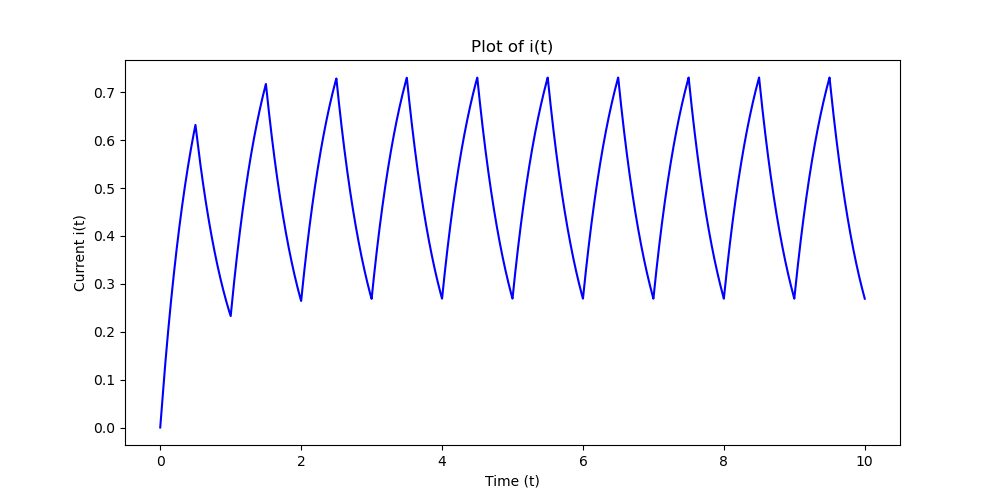
\includegraphics[width=0.8\linewidth]{figs/complete-fourier.png}
    \caption{Circuit Response using Fourier Series}
    \label{fig:enter-label}
\end{figure}
% Chapter Template

\chapter{Steady State Analysis}

\label{Chapter2}

\lhead{Chapter 2. \emph{Steady State Response Analysis Using Frequency Response}} 

If one is interested in the steady state response only, an easier route would to use the frequency response of the system.
\section{Frequency Response }
    Suppose the input to a circuit is characterized by the following Fourier series,
    \begin{align*}
       V_{i} = V_{i, dc} + \sum C_n e^{j\omega nt} 
    \end{align*}
    The output current can be characterized by a Fourier series like the following,
    \begin{align*}
       I_{o} = I_{o, dc} + \sum C_{n}^{\prime}  e^{j\omega nt} 
    \end{align*}
   What we are interested in is a function of the angular frequency which can relate $C_n$ and $C_{n}^\prime$
   \begin{align*}
       C_n ^\prime = H\brak{j\omega} \cdot C_n
   \end{align*}
   The function H, commonly known as the \texttt{transfer function}, can be calculated easily by treating the quantities $C_n e^{j\omega nt}$ as the input voltage phasor and $C_n^\prime e^{j\omega nt}$ as the corresponding output phasor. 
   \begin{align*}
       \vec{I}_{o,n} = H\brak{jw} \cdot \vec{V}_{i,n}
   \end{align*}
\section{Calculating the transfer function}
   \begin{figure}[!ht]
        \centering
        \resizebox{0.5\textwidth}{!}{%
        \begin{circuitikz}
        \tikzstyle{every node}=[font=\LARGE]
        \draw (3.5,15.75) to[R] (7,15.75);
        \draw (6,15.75) to[L ] (9.25,15.75);
        \draw (9.25,12) to[square voltage source, sources/symbol/rotate=auto] (3.5,12);
        \draw (3.5,15.75) to[short] (3.5,12);
        \draw (9.25,15.75) to[short] (9.25,12);
        \node [font=\LARGE] at (6.5,11) {$\vec{V}_{i, n}$};
        \draw [->, >=Stealth] (4,16.25) -- (8.5,16.25);
        \node [font=\LARGE] at (6.25,16.75) {$\vec{I}_{o,n}$};
        \node [font=\LARGE] at (5.25,15) {$R$};
        \node [font=\LARGE] at (7.75,15) {$j\omega L$};
        \end{circuitikz}
        }%
    \end{figure}
    The total input impedance is given by 
    \begin{align*}
        \vec{Z} = R + \frac{1}{j\omega C}
    \end{align*}    
    Therefore the output current is given by,
    \begin{align*}
        \vec{I}_{o,n} = \frac{\vec{V}_i}{\vec{Z}} &= \vec{V}_{i,n}\brak{\frac{1}{R + {jn\omega L}}}\\
    \end{align*}
    From this we can get the transfer function, 
    \begin{align*}
        H\brak{jn\omega} = \frac{\vec{I}_{o,n}}{\vec{V}_{i,n}} = \frac{1}{R + {jn\omega L}}
    \end{align*}
\section{Applying the Frequency Response Method}
    From the previous analysis,
    \begin{align*}
        V_i = A\alpha + \sum \brak{\frac{A}{n\pi}\sin\brak{n\pi\alpha}e^{-jn\pi\alpha}}e^{jn\omega t}
    \end{align*}
    Using the transfer function derived previously, 
    \begin{align*}
        I_o = \frac{A\alpha}{R}  + \sum \brak{\frac{A}{n\pi}\frac{\sin\brak{n\pi\alpha}}{R + {jn\omega L}}e^{-jn\pi\alpha}}e^{jn\omega t}
    \end{align*}
    Graphed out, it looks something like this
    \begin{figure}
        \centering
        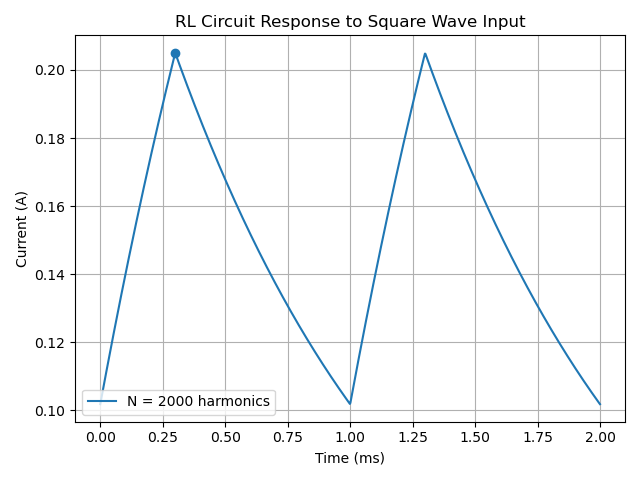
\includegraphics[width=0.8\linewidth]{figs/steady-state.png}
        \caption{Steady state solution to our differential equation}
    \end{figure}
\section{Conclusions}
    The similarity of the solution to a triangular wave is to be expected due to the following fact, 
    \begin{align*}
        \frac{d}{dt}\brak{\text{triangular wave}} = \text{square wave}
    \end{align*}
    In our differential equation as $R \rightarrow 0$, we get,
    \begin{align*}
        \frac{di}{dt} = \frac{V\brak{t}}{L}
    \end{align*}
    which validates our observation.
    \newline
    Coming to the peak deviations from the DC component of the response, the peaks are always located at $t = nT + \alpha T$. So
    \begin{align*}
        \Delta I_o &= \left \|\sum \brak{\frac{A}{n\pi}\frac{\sin\brak{n\pi\alpha}}{R + {jn\omega L}}e^{-jn\pi\alpha}}e^{jn\omega \alpha T} \right\|\\
        &=  \left\| \sum\brak{\frac{A}{n\pi}\frac{\sin\brak{n\pi\alpha}}{R + {jn\omega L}}e^{jn\pi\alpha}} \right \| \\
    \end{align*}
    It is not clear on initial inspection what this series will converge to. So we seek a simpler method to get these offset values.
    \subsection{A simpler way}
    We notice that for system to attain steady state, the current at the starting and end of each cycle should be the same.
    Suppose $I_{cy}$ is the current at the beginning of a cycle in steady state. The inductor will charge through the resistor for time $\Delta t = \alpha T$. So the current at the end of $\alpha T$ seconds will be,
    \begin{align*}
        I_{\alpha T} = \frac{A}{R} + \brak{I_{cy} - \frac{A}{R}}e^{\frac{-R\alpha T}{L}}
    \end{align*}
    For the remainder of the cycle, the inductor discharges. Thus, the current at the end of the cycle is,
    \begin{align*}
        I_{cy}^{\prime} = I_{\alpha T}e^{\frac{-R\brak{T-\alpha T}}{L}}\\
    \end{align*}
    But,
    \begin{align*}
        I_{cy} = I_{cy}^\prime 
    \end{align*}
    On simplification, 
    \begin{align*}
        I_{cy} = \frac{A}{R}e^{\frac{-RT}{L}}\brak{\frac{e^{\frac{R\alpha T}{L}} - 1}{1-e^{\frac{-RT}{L}}}}
    \end{align*}

    From this we calculate the maximum offset to be,
    \begin{align*}
       \Delta I_{max} &= \frac{A}{R} + \brak{I_{cy} - \frac{A}{R}}e^{\frac{-R\alpha T}{L}} - I_{cy}\\
        &= \frac{A}{R}\brak{1 - e^{\frac{-R\alpha T}{L}}} + I_{cy}\brak{e^{\frac{-R\alpha T}{L}} - 1} \\
        &= \brak{1 - e^{\frac{-R\alpha T}{L}}}\brak{\frac{A}{R} - I_{cy}}\\
        &=\frac{A}{R}\brak{1 - e^{\frac{-R\alpha T}{L}}}\brak{1 - \brak{\frac{e^{\frac{R\alpha T}{L}} - 1}{e^{\frac{RT}{L}} - 1}}}\\
        \Delta I_{max} &=\frac{A}{R}\brak{1 - e^{\frac{-R\alpha T}{L}}} \brak{\frac{e^{\frac{RT}{L}}-e^{\frac{R\alpha T}{L}}}{e^{\frac{RT}{L}} - 1}}\\
    \end{align*}

    No wonder we could not find a closed solution previously!\\
    \quad\newline
    So the dependence of the amplitude of oscillation about mean value can be summarized in the following way,
    \begin{enumerate}
        \item Increasing the time period will increase the amplitude of deviations.
        \item Increasing the duty ratio upto 0.5 also increases and after that, it will decrease .
        \item Increasing either the resistance or the inductance will reduce the amplitude of the deviations.
    \end{enumerate}
    \begin{figure}
        \centering
        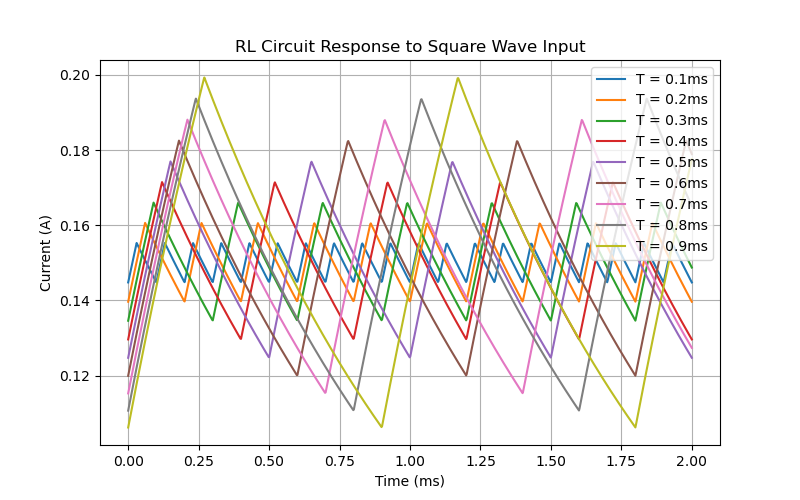
\includegraphics[width=0.8\linewidth]{figs/time-period_variation.png}
        \caption{Variation of amplitude of oscillations with time period}
        \label{fig:enter-label}
    \end{figure}
    \begin{figure}
        \centering
        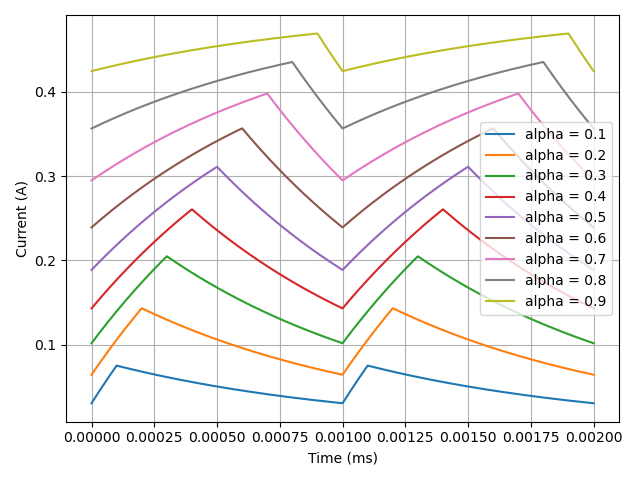
\includegraphics[width=0.8\linewidth]{figs/alpha_variation.png}
        \caption{Variation of amplitude of oscillations with duty ratio}
        \label{fig:enter-label}
    \end{figure} 
% Chapter Template

\chapter{Numerical Analysis} % Main chapter title

\label{Chapter3} % Change X to a consecutive number; for referencing this chapter elsewhere, use \ref{ChapterX}

\lhead{Chapter 3. \emph{Numerical Analysis}} % Change X to a consecutive number; this is for the header on each page - perhaps a shortened title

\section{Linear Stability Analysis}
Let's consider the following for analyzing the methods:
    \begin{itemize}
        \item Resistor R=10 $\Omega$
        \item Inductor L=1mH
        \item For the input square wave $v_{in}$:\\
        Amplitude $v_{0}=5V$\\
        Time Period T=1ms\\
        Duty Ratio $\alpha$ =0.5
    \end{itemize}
    The square wave input:\\
    \[
        V(t) =
        \begin{cases}
        5 \, \text{V}, & \text{if } 0 \leq t < 0.5 \, \text{ms} \\
        0 \, \text{V}, & \text{if } 0.5 \, \text{ms} \leq t < 1 \, \text{ms}
        \end{cases}
    \]
    and the governing equation after substituting R and L values is \[\frac{di(t)}{dt}=1000v_{in}(t)-10000i(t)\]\\
    For the RL equation the eigenvalue $\lambda=-\frac{R}{L}=-10000$.\\
\begin{enumerate}
    \item \textbf{RK-2}\\
    The stability function for RK-2 is:
    \begin{equation}
        R(z)=1+z+ \frac{z^2}{2}
    \end{equation}
    where $z=h \lambda$ and the condition for stability is $|R(z)| \leq 1$.\\
    On solving the equation $\lambda =-\frac{R}{L}$.
    Substituting the value of $\lambda$ into stability condition:
    \begin{equation}
        |1-h \frac{R}{L}+\frac{(h \frac{R}{L})^2}{2}| \leq 1
    \end{equation}
    
    Now, substituting $\lambda=-10000$ into the stability condition:
    \begin{equation}
        |1+h(-10000)+\frac{(h(-10000))^2}{2}| \leq 1
    \end{equation}
    \textbf{Conclusion:} RK-2 is conditionally stable for \( h \leq 0.0002 \, \text{s} \)

    
    \item \textbf{Forward Euler}\\
    The Forward Euler method approximates the solution as:
    \begin{equation}
        i_{n+1} = i_n + h \lambda i_n = (1 + h \lambda) i_n.
    \end{equation}
    The stability condition is:
    \begin{equation}
        |1 + h \lambda| \leq 1.
    \end{equation}
    Substituting \( \lambda = -10000 \) from the example before:
    \begin{equation}
        |1 - 10000 h| \leq 1 \implies h \leq 0.0002 \, \text{s}.
    \end{equation}
    \textbf{Conclusion:} Forward Euler is conditionally stable for \( h \leq 0.0002 \, \text{s} \).
    

    \item \textbf{Backward Euler}\\
    The Backward Euler method approximates the solution as:
    \begin{equation}
        i_{n+1} = i_n + h \lambda i_{n+1} \implies i_{n+1} = \frac{i_n}{1 - h \lambda}.
    \end{equation}
    The stability condition is:
    \begin{equation}
        \left| \frac{1}{1 - h \lambda} \right| \leq 1.
    \end{equation}
    Since \( \lambda = -10000 \), this becomes:
    \begin{equation}
        \left| \frac{1}{1 + 10000 h} \right| \leq 1,
    \end{equation}
    which is always true for \( h > 0 \).\\
    \textbf{Conclusion:} Backward Euler is unconditionally stable.


    \item \textbf{RK-4}\\
    The RK-4 method has the stability function:
    \begin{equation}
        R(z) = 1 + z + \frac{z^2}{2} + \frac{z^3}{6} + \frac{z^4}{24}, \quad z = h \lambda.
    \end{equation}
    The stability condition is:
    \begin{equation}
        |R(z)| \leq 1.
    \end{equation}
    Substituting \( \lambda = -10000 \):
    \begin{equation}
        |R(-10000 h)| \leq 1 \implies h \leq 0.0002785 \, \text{s}.
    \end{equation}
    \textbf{Conclusion:} RK-4 is conditionally stable for \( h \leq 0.0002785 \, \text{s} \).


    \item \textbf{Trapezoidal Method}\\
    The Trapezoidal method approximates the solution as:
    \begin{equation}
        i_{n+1} = i_n + \frac{h}{2} (\lambda i_n + \lambda i_{n+1}) \implies i_{n+1} = \frac{1 + \frac{h \lambda}{2}}{1 - \frac{h \lambda}{2}} i_n.
    \end{equation}
    The stability condition is:
    \begin{equation}
        \left| \frac{1 + \frac{h \lambda}{2}}{1 - \frac{h \lambda}{2}} \right| \leq 1.
    \end{equation}
    Substituting \( \lambda = -10000 \):
    \begin{equation}
        \left| \frac{1 - 5000 h}{1 + 5000 h} \right| \leq 1,
    \end{equation}
    which is always true for \( h > 0 \).\\
    \textbf{Conclusion:} The Trapezoidal method is unconditionally stable.

\end{enumerate}

\section{Showcase of Stability Regions}
\begin{figure}[H]
  \centering
  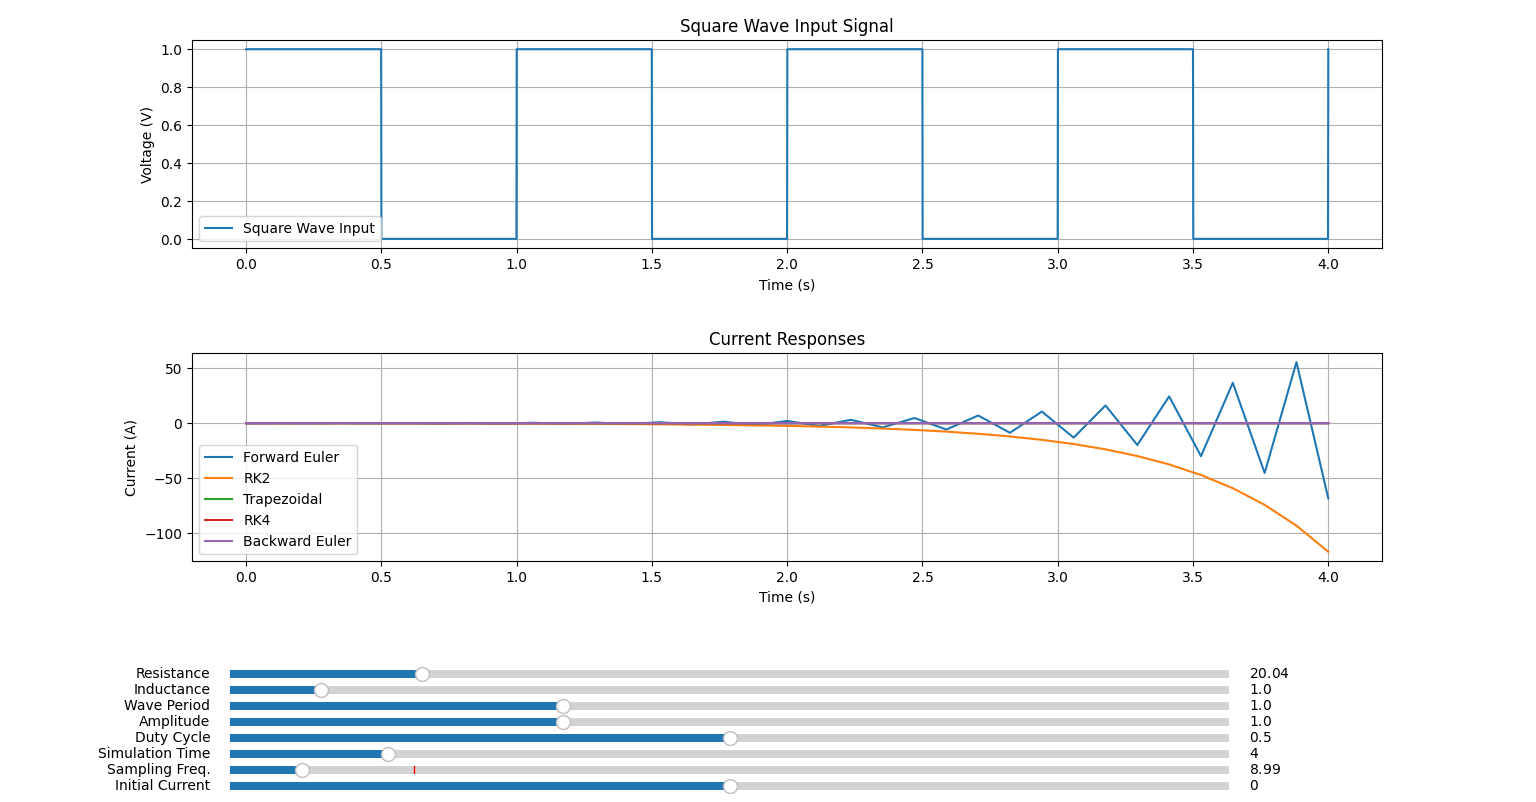
\includegraphics[width=\textwidth]{figs/instability_fwd_euler.png}
  \caption{Instability of the Forward Euler method for a step size that violates the stability condition.}
  \label{fig:instability_forward_euler}
\end{figure}

\begin{figure}[H]
  \centering
  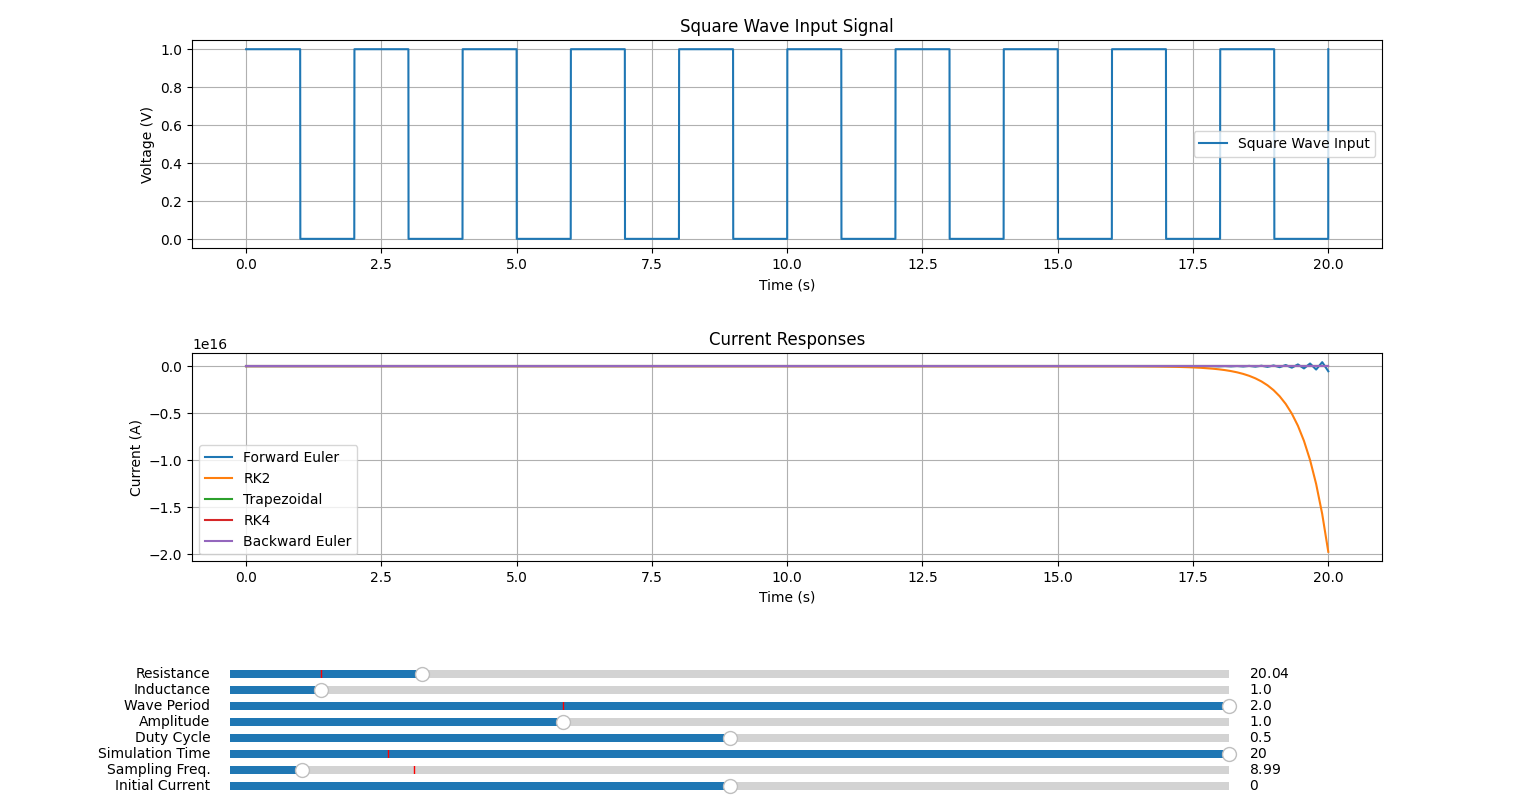
\includegraphics[width=\textwidth]{figs/instability_rk2.png}
  \caption{Instability behavior of RK2 (Heun's) method when the step size is too large.}
  \label{fig:instability_rk2}
\end{figure}


\begin{figure}[H]
  \centering
  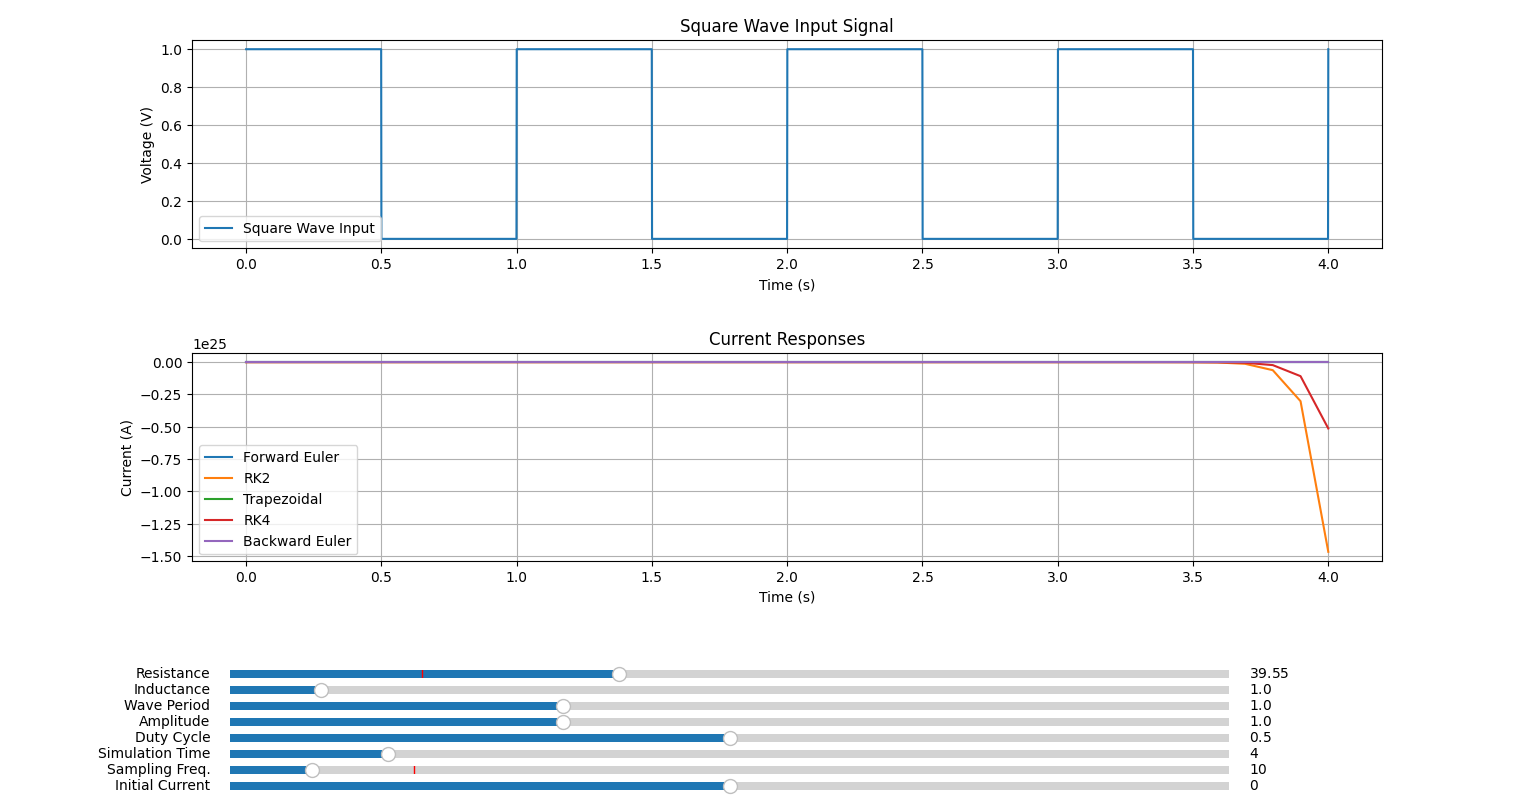
\includegraphics[width=\textwidth]{figs/instability_rk4.png}
  \caption{Instability behavior of RK4 when the step size exceeds the stability region (bounded region).}
  \label{fig:instability_rk4}
\end{figure}
\section{Local and Global Truncation Error}
\begin{figure}[H]
  \centering
  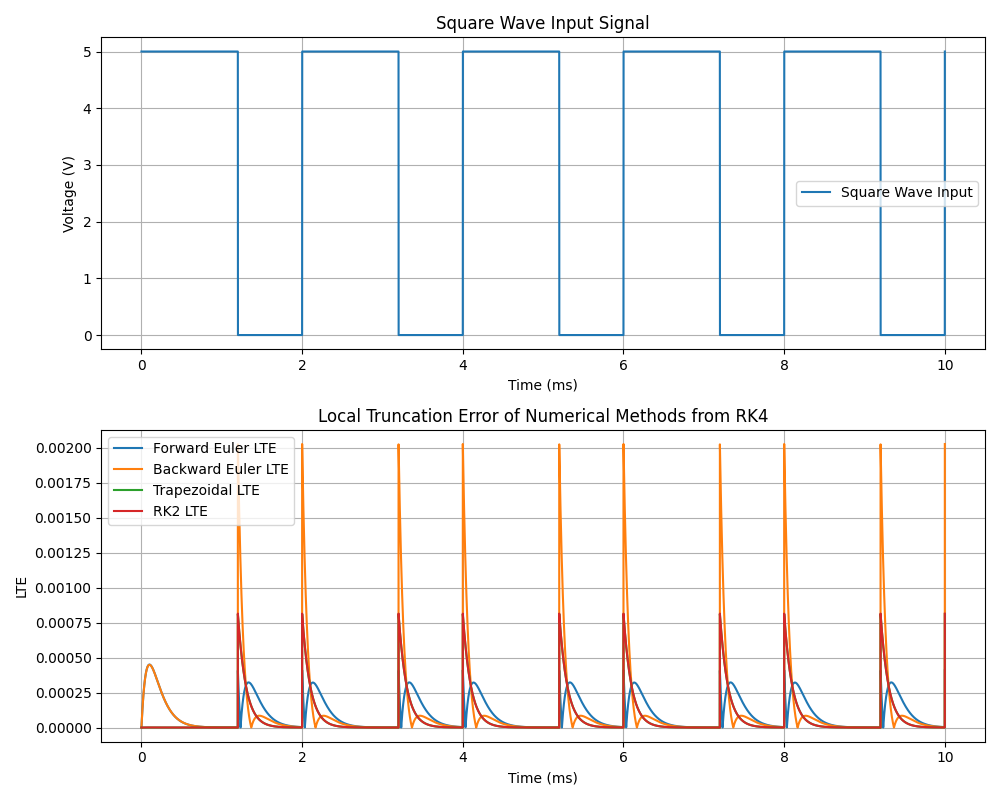
\includegraphics[width=\textwidth]{figs/local_error.png}
  \caption{Local truncation error at each sample point for selected values of $R$, $L$, and the sampling rate.}
  \label{fig:local_error}
\end{figure}

\begin{figure}[H]
  \centering
  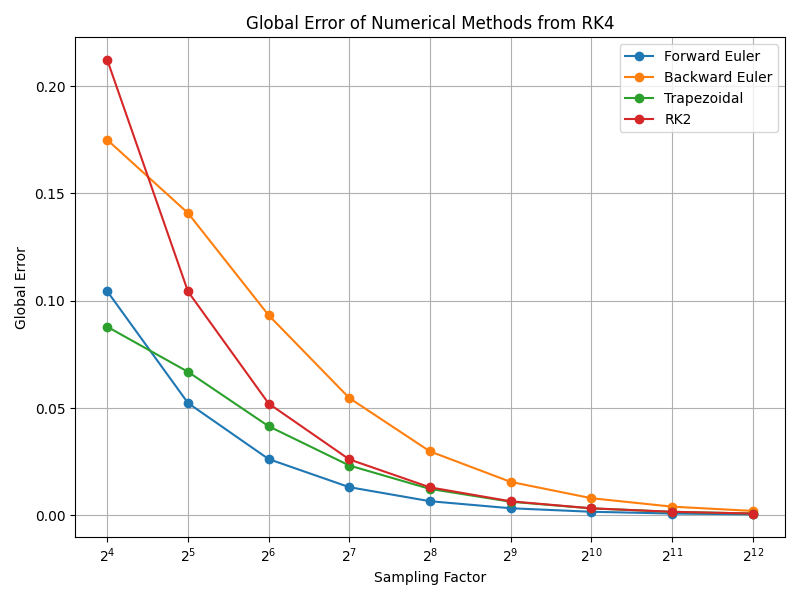
\includegraphics[width=\textwidth]{figs/global_error.png}
  \caption{Global error versus the sampling factor. The RK4 method is used as the reference due to its higher order accuracy ($O(h^4)$).}
  \label{fig:global_error}
\end{figure}
\section{Comparison of Computational Times}
\begin{figure}[H]
  \centering
  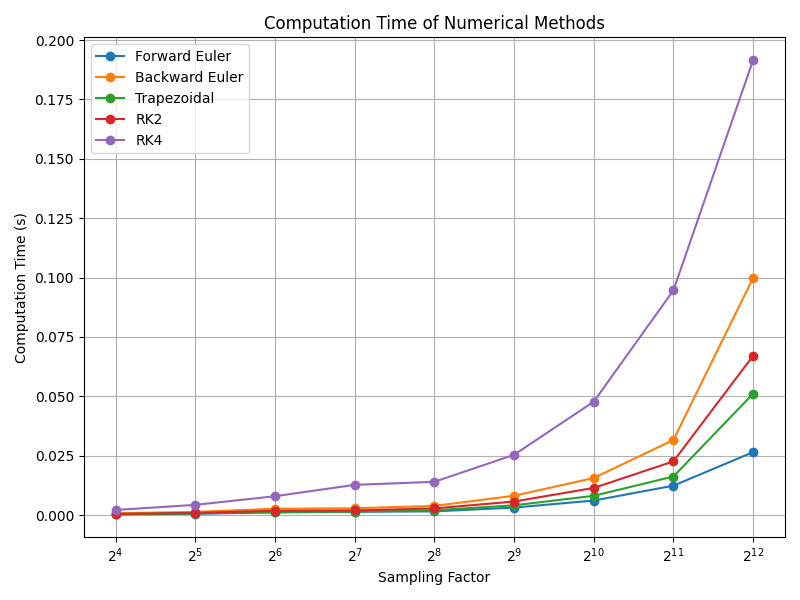
\includegraphics[width=\textwidth]{figs/computation_time.png}
  \caption{Computational times (y-axis) versus sampling factors (x-axis) for the different methods.}
  \label{fig:comp_times}
\end{figure}


% Chapter Template

\chapter{Convergence - Uniform, Absolute and Pointwise}

\label{Chapter4}

\lhead{Chapter 4. \emph{Convergence of Current Fourier Series}} 


\section{What is Convergence?}
Convergence refers to whether a sequence of approximations gets closer to a target value. For a Fourier series, convergence means that the series representation of a function behaves like the function as we add more terms. That is, the partial sum:
\begin{equation}
S_N(x) = a_0 + \sum_{n=1}^{N} (a_n \cos(nx) + b_n \sin(nx))
\end{equation}
should get closer and closer to $f(x)$ as $N \to \infty$.


\section{Understanding Convergence in Fourier Series}

When we approximate a function $f(x)$ using its Fourier series, we want to know how well the series actually represents $f(x)$. The term *"convergence"* describes whether and how the sum of the Fourier series approaches the function. There are three main types of convergence we study:\\\\
1. *Pointwise Convergence* – Does the Fourier series converge to $f(x)$ at each point?\\
2. *Uniform Convergence* – Does the convergence happen evenly across the entire interval?\\
3. *Absolute Convergence* – Does the sum of the absolute values of the terms converge?\\

Each of these has different implications for how well the Fourier series represents $f(x)$, and understanding them helps in analyzing how Fourier series behave in practical applications.

\section{Pointwise Convergence}
\subsection{Definition}
A sequence of functions $S_N(x)$ converges \textit{pointwise} to a function $f(x)$ if for each fixed $x$, the sequence $S_N(x)$ gets arbitrarily close to $f(x)$ as $N \to \infty$, i.e.,
\[
\lim_{N \to \infty} S_N(x) = f(x).
\]
For a Fourier series, this means that at each specific point $x$, the sum of the first $N$ terms of the series gets closer and closer to $f(x)$ as $N$ increases.

\subsection{Mathematical Proof of Pointwise Convergence for Fourier Series}
Consider the Fourier series of a function $f(x)$:
\[
S_N(x) = \sum_{n=-N}^{N} c_n e^{j n \omega x}.
\]
We analyze whether this series converges to $f(x)$ for each $x$. The *Dirichlet conditions* guarantee pointwise convergence almost everywhere if:

1. $f(x)$ is piecewise continuous (it has a finite number of discontinuities).
2. $f(x)$ is piecewise smooth (both $f(x)$ and $f'(x)$ are piecewise continuous).

If these conditions are met, the Fourier series converges to $f(x)$ at points where $f(x)$ is continuous. However, at discontinuities, the Fourier series converges to the *midpoint* of the left-hand and right-hand limits:
\[
S_N(x) \to \frac{f(x^+) + f(x^-)}{2}.
\]
This is known as the *Gibbs phenomenon*, where the Fourier series overshoots near discontinuities.

\section{Uniform Convergence}
\subsection{Definition}
A Fourier series converges \textit{uniformly} to $f(x)$ if the error between $S_N(x)$ and $f(x)$ can be made arbitrarily small for all $x$ at the same time, i.e.,
\[
\sup_{x} |S_N(x) - f(x)| \to 0 \text{ as } N \to \infty.
\]
This means that no matter where you look, the difference between the partial sum $S_N(x)$ and $f(x)$ is consistently small across the entire interval.

\subsection{Why Fourier Series May Not Converge Uniformly}
If a Fourier series is to converge uniformly, it must satisfy the Weierstrass M-test, which roughly states that the terms of the series must decrease in a controlled way. However, if $f(x)$ has a discontinuity, uniform convergence fails due to the Gibbs phenomenon—the oscillations near the discontinuity remain significant even as $N \to \infty$.

A key theorem states that if a Fourier series converges uniformly, then it must also converge absolutely. Since Fourier series do not always converge absolutely, they often fail to be uniformly convergent.

\section{Absolute Convergence}
\subsection{Definition}
A series $\sum a_n$ is said to be \textit{absolutely convergent} if the series of absolute values $\sum |a_n|$ also converges.

For a Fourier series, absolute convergence means:
\[
\sum_{n=-\infty}^{\infty} |c_n| < \infty.
\]
This ensures that the series is well-behaved and guarantees uniform convergence.

\subsection{Why Most Fourier Series Do Not Converge Absolutely}
The Fourier coefficients $c_n$ of a function $f(x)$ typically decay as $\frac{1}{n}$ or slower. The harmonic series:
\[
\sum_{n=1}^{\infty} \frac{1}{n}
\]
diverges, which means that most Fourier series do *not* converge absolutely.



\section{Comparison of Convergence Types}
\begin{table}[h]
    \centering
    \renewcommand{\arraystretch}{1.3}
    \begin{tabular}{p{4cm} p{3cm} p{5cm} p{4cm}}
        \toprule
        \textbf{Convergence Type} & \textbf{Strength} & \textbf{Works for Discontinuous Functions?} & \textbf{Key Condition} \\
        \midrule
        Pointwise   & Weak  & Yes, but oscillates at jumps  & $S_N(x) \to f(x)$ at each point \\
        \midrule
        Uniform    & Medium  & No (fails at discontinuities) & $\sup |S_N(x) - f(x)| \to 0$ \\
        \midrule
        Absolute   & Strong  & Rarely (only for fast-decaying coefficients) & $\sum |a_n| + |b_n| < \infty$ \\
        \bottomrule
    \end{tabular}
    \caption{Comparison of convergence types in Fourier series.}
\end{table}

\section{Convergence}
Analysis of the convergence properties of the complex Fourier series representation of the current response in a series RL circuit subjected to a square wave input. We examine three types of convergence:
\begin{itemize}
  \item \textbf{Pointwise Convergence}
  \item \textbf{Uniform Convergence}
  \item \textbf{Absolute Convergence}
\end{itemize}
Each section includes step-by-step proofs with explicit integration and simplifications.

\section{Complex Fourier Series Representation of RL Circuit Response}
The RL circuit is governed by the differential equation:
\begin{equation}
L \frac{di}{dt} + R i = V(t),
\end{equation}
where $L$ is the inductance, $R$ is the resistance, and $i(t)$ is the circuit current.

For a square wave voltage input with period $T$, we expand it into its complex Fourier series:
\begin{equation}
V(t) = A\alpha + \sum_{k=-\infty}^{\infty} \frac{A}{\pi k} \sin (\pi k \alpha)e^{-j \pi k \alpha} e^{j k \omega t}, \quad \omega = \frac{2\pi}{T}.
\end{equation}
The Fourier coefficients are given by:
\begin{equation}
C_k = \frac{1}{T} \int_{0}^{T} V(t) e^{-j k \omega t} dt.
\end{equation}

Using this representation, we obtain the Fourier series for the circuit current:
\begin{equation}
i(t) = \frac{A \alpha}{R} \left(1 - e^{-\frac{R T}{L}}\right) + \sum_{k=-\infty}^{\infty} \left( \frac{A \sin (\pi k \alpha) e^{-j \pi k \alpha}}{\pi k (L j k \omega + R)} \right) \left(e^{j k \omega t} - e^{-\frac{R T}{L}}\right).
\end{equation}

\section{Pointwise Convergence}
Pointwise convergence requires that:
\begin{equation}
\lim_{N \to \infty} S_N(t) = i(t),
\end{equation}
where $S_N(t)$ is the $N$-term partial sum of the Fourier series. According to Dirichlet's theorem, a Fourier series converges pointwise to the function value wherever the function is continuous. At points of discontinuity, the Fourier series converges to the average of the left-hand and right-hand limits:
\begin{equation}
\lim_{N \to \infty} S_N(t) = \frac{V(t^+) + V(t^-)}{2}.
\end{equation}
Since the square wave has jump discontinuities, the Fourier series representation of $V(t)$ exhibits the Gibbs phenomenon.

\section{Uniform Convergence}
Uniform convergence requires:
\begin{equation}
\sup_{t \in [0,T]} |S_N(t) - i(t)| \to 0 \quad \text{as} \quad N \to \infty.
\end{equation}
The Weierstrass M-test can be used to determine uniform convergence. If there exists a sequence $M_n$ such that:
\begin{equation}
|I_n| \leq M_n \quad \text{and} \quad \sum M_n < \infty,
\end{equation}
then the series converges uniformly. However, due to the Gibbs phenomenon and oscillatory nature of the Fourier series, the error remains nonzero near discontinuities, proving that uniform convergence fails.

\section{Absolute Convergence}
A Fourier series converges absolutely if:
\begin{equation}
\sum_{k=-\infty}^{\infty} |I_k| < \infty.
\end{equation}
Since $I_k \sim \frac{1}{k}$ for large $k$, the series behaves like the harmonic series:
\begin{equation}
\sum \frac{1}{k},
\end{equation}
which is known to diverge. Hence, the Fourier series does not converge absolutely.

\section{Conclusion}
The Fourier series representation of the RL circuit response exhibits different types of convergence properties:
\begin{itemize}
  \item \textbf{Pointwise Convergence}: The Fourier series converges pointwise everywhere except at discontinuities, where it converges to the average of the left and right limits due to the Gibbs phenomenon.
  \item \textbf{Uniform Convergence}: The Fourier series does not converge uniformly because the Gibbs phenomenon introduces a persistent oscillatory error near discontinuities.
  \item \textbf{Absolute Convergence}: The Fourier series does not converge absolutely since its terms decay as $\frac{1}{k}$, leading to divergence of the harmonic series.
\end{itemize}
These results indicate that while the Fourier series accurately represents the RL circuit response in a pointwise sense, its lack of uniform and absolute convergence affects practical considerations such as truncation error and approximation quality near discontinuities.
 
% Chapter Template

\chapter{Supercharging our Numerical Methods}

\label{Chapter5} % Change X to a consecutive number

\lhead{Chapter 5. \emph{Faster Computations with Parareal}}
\section{Parareal}
    The hunger for speed and accuracy can't be satisfied without using all our computer's resource to crunch the numbers. The most obvious way to do this is is to run our code on separate threads concurrently. 
    
\subsection{Algorithm Description}
The Parareal Algorithm follows these steps:
\begin{enumerate}
    \item Compute a "bad" approximation to the solution using the coarse solver.
    \item Compute corrections in parallel using the fine solver.
    \item Update the solution iteratively using a predictor-corrector approach until convergence is achieved.
\end{enumerate}

\subsection{Mathematical Formulation}
Consider a differential equation of the form:
\begin{equation}
    \frac{du}{dt} = f(u,t), \quad u(0) = u_0.
\end{equation}
The time domain is divided into intervals, and two solvers are defined:
\begin{itemize}
    \item A coarse solver, $C_j^k$, which provides an initial guess.
    \item A fine solver, $F_j^k$, which refines the solution in parallel.
\end{itemize}
The iteration formula is given by:
\begin{align*}
    C_{j+1}^{k+1} = C_{j+1}^k + F_j^k - C_j^k.
\end{align*}
The method is captured beautifully by this 
\href{https://upload.wikimedia.org/wikipedia/commons/transcoded/b/b5/Parareal_Animation.ogv/Parareal_Animation.ogv.720p.vp9.webm}{animation} from Wikipedia.
\subsection{Benchmarks}
The source code and benchmarking code is written in GoLang.
The following results are taken when the baseline RK4 solution runs with 1,00,000 iterations while the Parareal solution runs with 1000 coarse steps and 200 fine sub-steps. So the Parareal solution computes 2X the number of points.
\newpage
\begin{verbatim}
go test -bench .  
goos: linux
goarch: amd64
pkg: example.com/greetings
cpu: AMD Ryzen 7 7730U with Radeon Graphics         
BenchmarkParareal-16                  84          14755702 ns/op
BenchmarkRK4-16                        2         745605400 ns/op
PASS
ok      example.com/greetings   3.482s
\end{verbatim}
This shows that the baseline RK4 method performs $\frac{745605400 }{14755702} \approx 50$ times slower !!
\begin{figure}
    \centering
    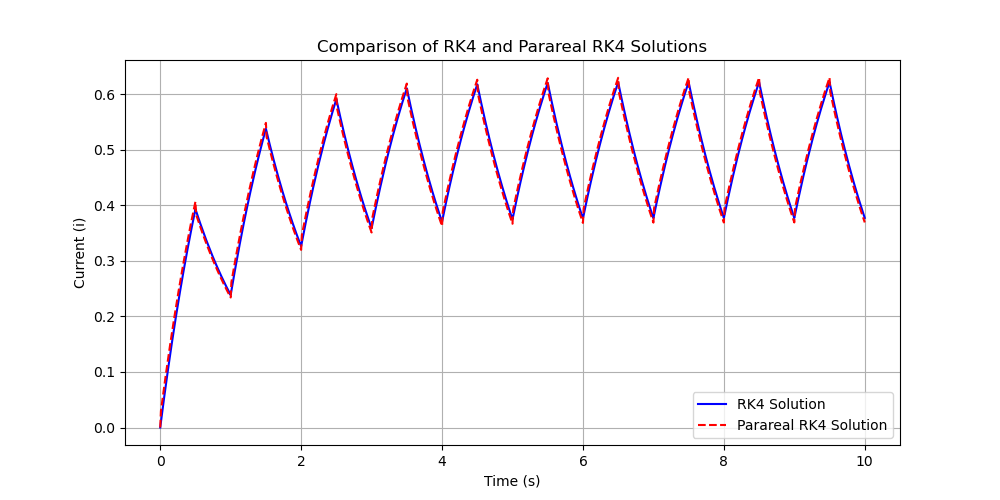
\includegraphics[width=0.8\linewidth]{figs/benchmark.png}
    \caption{Parareal v.s RK4}
\end{figure} 
% Chapter Template

\chapter{Efficiency Analysis}

\label{Chapter6}

\lhead{Chapter 6. \emph{Efficiency Analysis}}
\section{Power Dissipation in Steady State}
    The calculations in this section are relevant for certain applications, which will be discussed later.
\subsection{Calculations}
    The current in steady state in the time interval $nT \le t \le nT + \alpha T$ is given by, 
    \begin{align*}
               I_{1} = \frac{A}{R} + \brak{I_{cy} - \frac{A}{R}}e^{\frac{-Rt}{L}}
    \end{align*}
    where $I_{cy} =\frac{A}{R}e^{\frac{-RT}{L}}\brak{\frac{e^{\frac{R\alpha T}{L}} - 1}{1-e^{\frac{-RT}{L}}}}
 $
    Energy dissipated in this interval is given by, 
    \begin{align*}
        E_1 &= \int_{0}^{\alpha T} I_1^2R dt\\
        &= \int_0^{\alpha T}\brak{\frac{A}{R} + \brak{I_{cy} - \frac{A}{R}}e^{\frac{-Rt}{L}}}^2 R\\
    \end{align*}
    Computing the integral, 
    \begin{align*}
        E_1 = \frac{A^2}{R} \alpha T + 2A \left(I_{cy} - \frac{A}{R}\right) \frac{L}{R} \left(1 - e^{\frac{-R\alpha T}{L}}\right) + \left(I_{cy} - \frac{A}{R}\right)^2 \frac{L}{2} \left(1 - e^{\frac{-2R\alpha T}{L}}\right)
    \end{align*}
    Coming to the rest of the cycle, the current is given by
    \begin{align*}
        I_{2} = I_{\alpha T}e^{\frac{-R\brak{t-\alpha T}}{L}}\\
    \end{align*}
    where $I_{\alpha T} =  \frac{A}{R} + \brak{I_{cy} - \frac{A}{R}}e^{\frac{-R\alpha T}{L}}
 $
 Again the power dissipated in the portion of the cycle is given by, 
 \begin{align*}
    E_2 &= \int_{0}^{\alpha T} I_2^2R dt\\
    &= \int_{0}^{\alpha T} \brak{I_{\alpha T}e^{\frac{-R\brak{t-\alpha T}}{L}}}^2R dt\\
 \end{align*}
 On computing the integral we get, 
 \begin{align*}
     E_2 = \frac{L}{2} I_{\alpha T}^2 \left(1 - e^{\frac{-2R\alpha T}{L}}\right)
 \end{align*}
 So the net power dissipated is $E_{net} = E_1 + E_2$.
 \subsection{Efficiency}
 Efficiency can be calculated using, 
 \begin{align*}
     \eta = \frac{\text{energy dissipated in one cycle}}{\text{energy supplied by source in one cycle}}
 \end{align*}
 where,
 \begin{align*}
    \text{Energy supplied by source in one cycle is} = A \alpha T
 \end{align*}
 \subsection{Results}
 It is worthy to take note here that for some values of the parameters the efficiency is quite high, 
 \begin{verbatim}
Amplitude = 10
alpha = 0.7
Time Period = 1e-06
Resistance = 10
Inductance = 1e-06
Efficiency = 0.8645496088953908    
 \end{verbatim}
This efficiency combined with smaller deviation size is ideal to use the circuit as a DC-DC converter, which the next topic of discussion.  
% Chapter Template

\chapter{Applications}

\label{Chapter7} % Change X to a consecutive number; for referencing this chapter elsewhere, use \ref{ChapterX}

\lhead{Chapter 7. \emph{Applications}}
\section{Power Dissipation in Steady State}
    The calculations in this section are relevant for certain applications, which will be discussed later.
\subsection{Calculations}
    The current in steady state in the time interval $nT \le t \le nT + \alpha T$ is given by, 
    \begin{align*}
               I_{1} = \frac{A}{R} + \brak{I_{cy} - \frac{A}{R}}e^{\frac{-Rt}{L}}
    \end{align*}
    where $I_{cy} =\frac{A}{R}e^{\frac{-RT}{L}}\brak{\frac{e^{\frac{R\alpha T}{L}} - 1}{1-e^{\frac{-RT}{L}}}}
 $
    Energy dissipated in this interval is given by, 
    \begin{align*}
        E_1 &= \int_{0}^{\alpha T} I_1^2R dt\\
        &= \int_0^{\alpha T}\brak{\frac{A}{R} + \brak{I_{cy} - \frac{A}{R}}e^{\frac{-Rt}{L}}}^2 R\\
    \end{align*}
    Computing the integral, 
    \begin{align*}
        E_1 = \frac{A^2}{R} \alpha T + 2A \left(I_{cy} - \frac{A}{R}\right) \frac{L}{R} \left(1 - e^{\frac{-R\alpha T}{L}}\right) + \left(I_{cy} - \frac{A}{R}\right)^2 \frac{L}{2} \left(1 - e^{\frac{-2R\alpha T}{L}}\right)
    \end{align*}
    Coming to the rest of the cycle, the current is given by
    \begin{align*}
        I_{2} = I_{\alpha T}e^{\frac{-R\brak{t-\alpha T}}{L}}\\
    \end{align*}
    where $I_{\alpha T} =  \frac{A}{R} + \brak{I_{cy} - \frac{A}{R}}e^{\frac{-R\alpha T}{L}}
 $
 Again the power dissipated in the portion of the cycle is given by, 
 \begin{align*}
    E_2 &= \int_{0}^{\alpha T} I_2^2R dt\\
    &= \int_{0}^{\alpha T} \brak{I_{\alpha T}e^{\frac{-R\brak{t-\alpha T}}{L}}}^2R dt\\
 \end{align*}
 On computing the integral we get, 
 \begin{align*}
     E_2 = \frac{L}{2} I_{\alpha T}^2 \left(1 - e^{\frac{-2R\alpha T}{L}}\right)
 \end{align*}
 So the net power dissipated is $E_{net} = E_1 + E_2$.
 \subsection{Efficiency}
 Efficiency can be calculated using, 
 \begin{align*}
     \eta = \frac{\text{energy dissipated in one cycle}}{\text{energy supplied by source in one cycle}}
 \end{align*}
 where,
 \begin{align*}
    \text{Energy supplied by source in one cycle is} = A \alpha T
 \end{align*}
 \subsection{Results}
 It is worthy to take note here that for some values of the parameters the efficiency is quite high, 
 \begin{verbatim}
Amplitude = 10
alpha = 0.7
Time Period = 1e-06
Resistance = 10
Inductance = 1e-06
Efficiency = 0.8645496088953908    
 \end{verbatim}
This efficiency combined with smaller deviation size is ideal to use the circuit as a DC-DC converter, which the next topic of discussion. 
\section{Application as DC-DC converters}
The circuit under inspection has some really direct use cases in the world of power electronics, namely \textbf{Buck Converters}.
\subsection{DC-DC Converters}
It is of critical importance to be able to change a supply DC voltage to different (higher or lower) DC value which is required for the operation of other systems. For example, PSUs in regular computers can provide DC 3.3, 5 and 12V DC voltage rails, but many modern microprocessors operate at voltages of the order of 1.83 V. So DC converters see use in the VRMs (Voltage Regulator Modules) of most modern motherboads.
\subsection{Design}
Buck converters is a DC-DC converter, which provides high efficiency and low ripple current. The converter is realized in the following form, 
\begin{figure}[!ht]
\centering
\resizebox{0.8\textwidth}{!}{%
\begin{circuitikz}
\tikzstyle{every node}=[font=\LARGE]
\draw (5.5,14.75) to[Tnmos, transistors/scale=1.02] (3,14.75);
\draw (3,14.75) to[american voltage source] (3,10.75);
\draw (3,10.75) to[short] (7.5,10.75);
\draw (7.5,10.75) to[D] (7.5,14.75);
\draw (7.5,14.75) to[L ] (12.5,14.75);
\draw (12.5,14.75) to[R] (12.5,11);
\draw (7.5,10.75) to[short] (12.5,10.75);
\draw (12.5,10.75) to[short] (12.5,11.25);
\draw (5.5,14.75) to[short] (7.5,14.75);
\draw (11,14.75) to[C] (11,10.75);
\node [font=\LARGE] at (1.5,12.75) {$V_s$};
\draw (12.5,14.75) to[short, -o] (14.25,14.75) ;
\draw (12.5,10.75) to[short, -o] (14.25,10.75) ;
\node [font=\LARGE] at (14.5,12.75) {$V_o$};
\end{circuitikz}
}%
\caption{Step Down Buck Converter}
\end{figure}
The MOSFET will act as a switch, switching at some very high frequency (typically 100 kHz to a few MHz). The current ripple is mellowed out even further by the large capacitance. So our analysis has left us with all the tools required to build an efficient buck converter- with low ripple current around our desired target voltage and minimal losses of energy - with real life use.
 
% Chapter Template

\chapter{Generalizing the Numerical Solution Using Fourier Solution}

\label{Chapter8} % Change X to a consecutive number; for referencing this chapter elsewhere, use \ref{ChapterX}

\lhead{Chapter 8. \emph{Generalizing the Fourier Numerical Solution}}

\section{Why?}
The problem with trying to plot out the fourier solution upto a certain number of frequencies is that, the fourier coefficients need to calculated separately for each type of problem. This is cumbersome and thus it is of value to search for a solution which id general and doesn't require us to hand-calculate each time.
\section{Solution - Fast Fourier Transform}
To solve this equation using the Fast Fourier Transform (FFT), we take the Fourier transform of both sides. The Fourier transform of a time-domain function $f(t)$ is defined as:
\begin{align}
    F(\omega) = \int_{-\infty}^{\infty} f(t) e^{-j\omega t} dt
\end{align}
Applying this to the given differential equation, we use the property that the Fourier transform of a derivative is given by:
\begin{align}
    \mathcal{F} \left( \frac{df}{dt} \right) = j\omega F(\omega)
\end{align}
Taking the Fourier transform of both sides:
\begin{align}
    L (j\omega I(\omega)) + R I(\omega) = V(\omega)
\end{align}
Rearranging for $I(\omega)$:
\begin{align}
    I(\omega) = \frac{V(\omega)}{R + j\omega L}
\end{align}
To obtain $i(t)$ in the time domain, we take the inverse Fourier transform:
\begin{align}
    i(t) = \mathcal{F}^{-1} \left( I(\omega) \right) = \mathcal{F}^{-1} \left( \frac{V(\omega)}{R + j\omega L} \right)
\end{align}
The inverse Fourier transform is computed numerically using the Inverse Fast Fourier Transform (IFFT) in practical implementations. This step allows us to reconstruct the time-domain current response from the frequency-domain solution.
To solve this equation using the Fast Fourier Transform (FFT), we take the Fourier transform of both sides. The Fourier transform of a time-domain function $f(t)$ is defined as:
\begin{align}
    F(\omega) = \int_{-\infty}^{\infty} f(t) e^{-j\omega t} dt
\end{align}
Applying this to the given differential equation, we use the property that the Fourier transform of a derivative is given by:
\begin{align}
    \mathcal{F} \left( \frac{df}{dt} \right) = j\omega F(\omega)
\end{align}
Taking the Fourier transform of both sides:
\begin{align}
    L (j\omega I(\omega)) + R I(\omega) = V(\omega)
\end{align}
Rearranging for $I(\omega)$:
\begin{align}
    I(\omega) = \frac{V(\omega)}{R + j\omega L}
\end{align}
To obtain $i(t)$ in the time domain, we take the inverse Fourier transform:
\begin{align}
    i(t) = \mathcal{F}^{-1} \left( I(\omega) \right) = \mathcal{F}^{-1} \left( \frac{V(\omega)}{R + j\omega L} \right)
\end{align}
The inverse Fourier transform is computed numerically using the Inverse Fast Fourier Transform (IFFT) in practical implementations. This step allows us to reconstruct the time-domain current response from the frequency-domain solution.
\section{Effects of sampling}
We use several different ranges of sampling frequency to see which is "good" enough.
     \begin{center}
          Below Nyquist Rate $(f_s < 2 f_{\max})$: 
     \end{center}
    \captionsetup{type=figure}
    \centering
    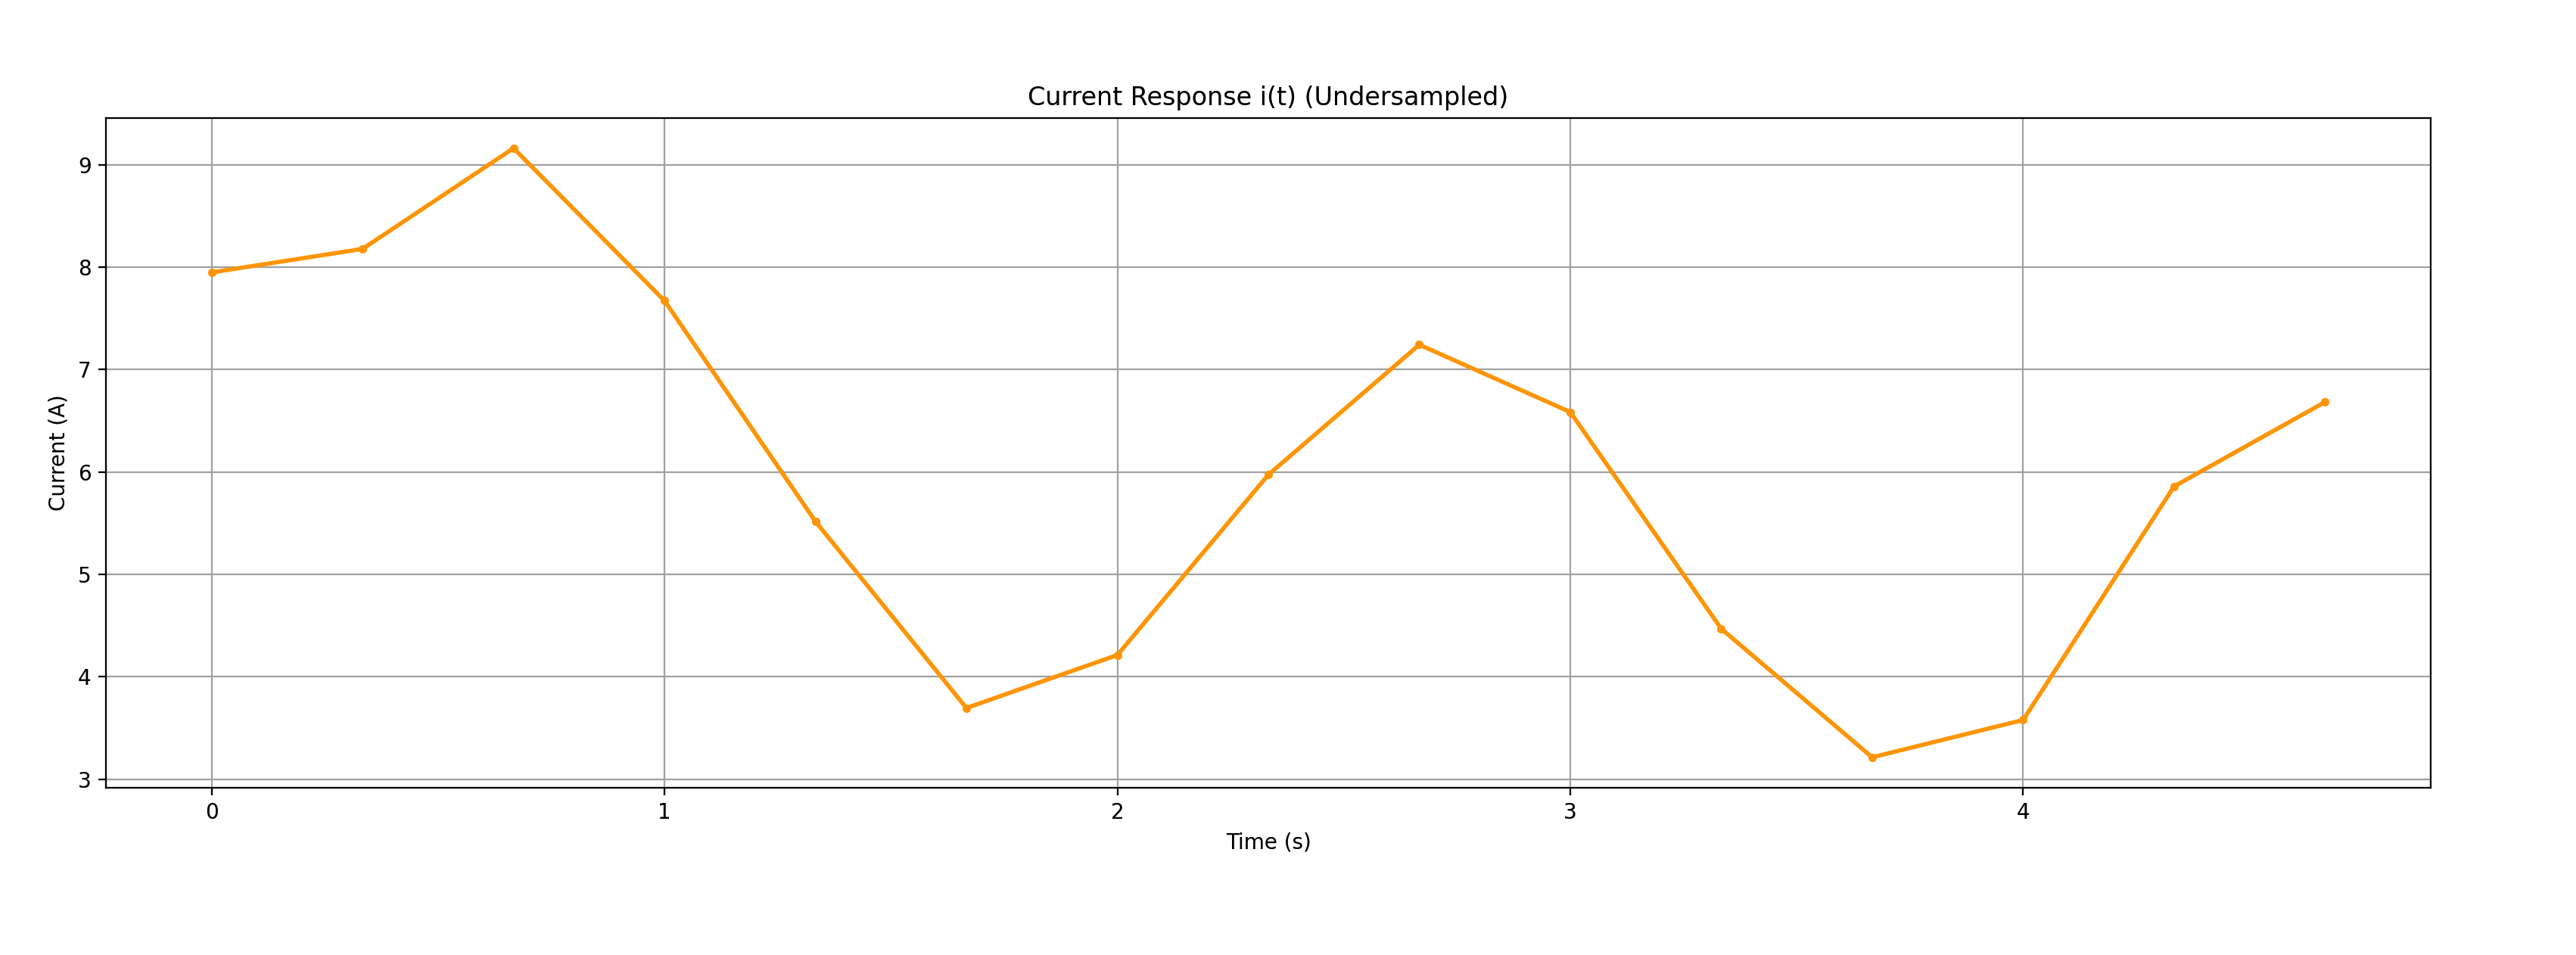
\includegraphics[width=0.6\textwidth]{figs/0_75f_ny.png}
    \caption{The current response for  $f_s < f_{ny}$   i.e, $(0.75*f_{ny})$}
    \label{fig:example}
      \begin{itemize}
          \item The square wave appears distorted, with missing transitions or incorrect duty cycle representation.
          \item The FFT spectrum shows incorrect frequency content.
      \end{itemize}
    \begin{center}  
      Slightly Above Nyquist Rate: 
    \end{center}
      
      \captionsetup{type=figure}
    \centering
    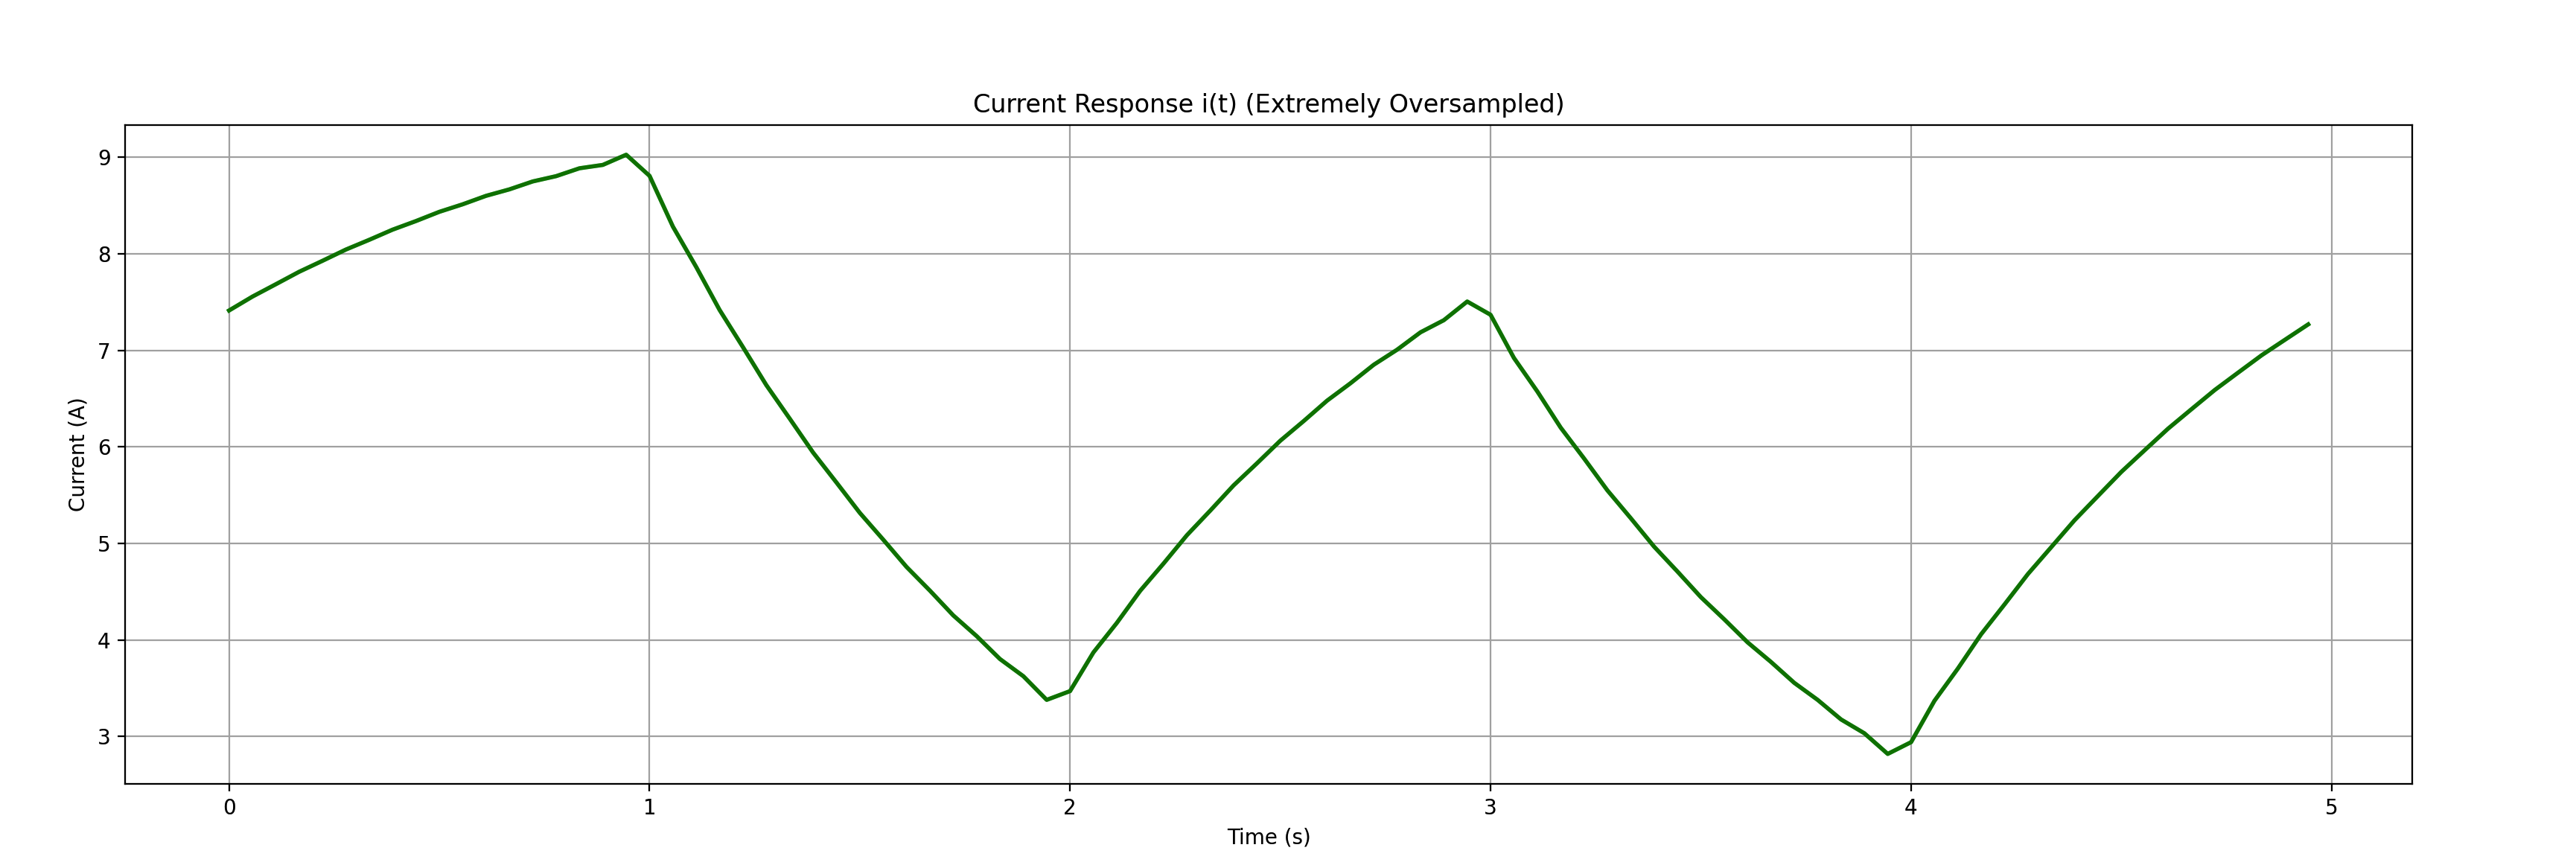
\includegraphics[width=0.6\textwidth]{figs/4_f_ny.png}
    \caption{The current response for  $f_s > f_{ny}$   i.e, $(4f_{ny})$}
    \label{fig:example}
    \begin{itemize}
        \item The waveform is well-preserved, and the current response $i(t)$ matches expected results.
        \item Harmonic content is properly captured.
    \end{itemize}
    \begin{center} 
     Very High Sampling Rate $(f_s \gg 2 f_{\max}):$
    \end{center}
     \captionsetup{type=figure}
    \centering
    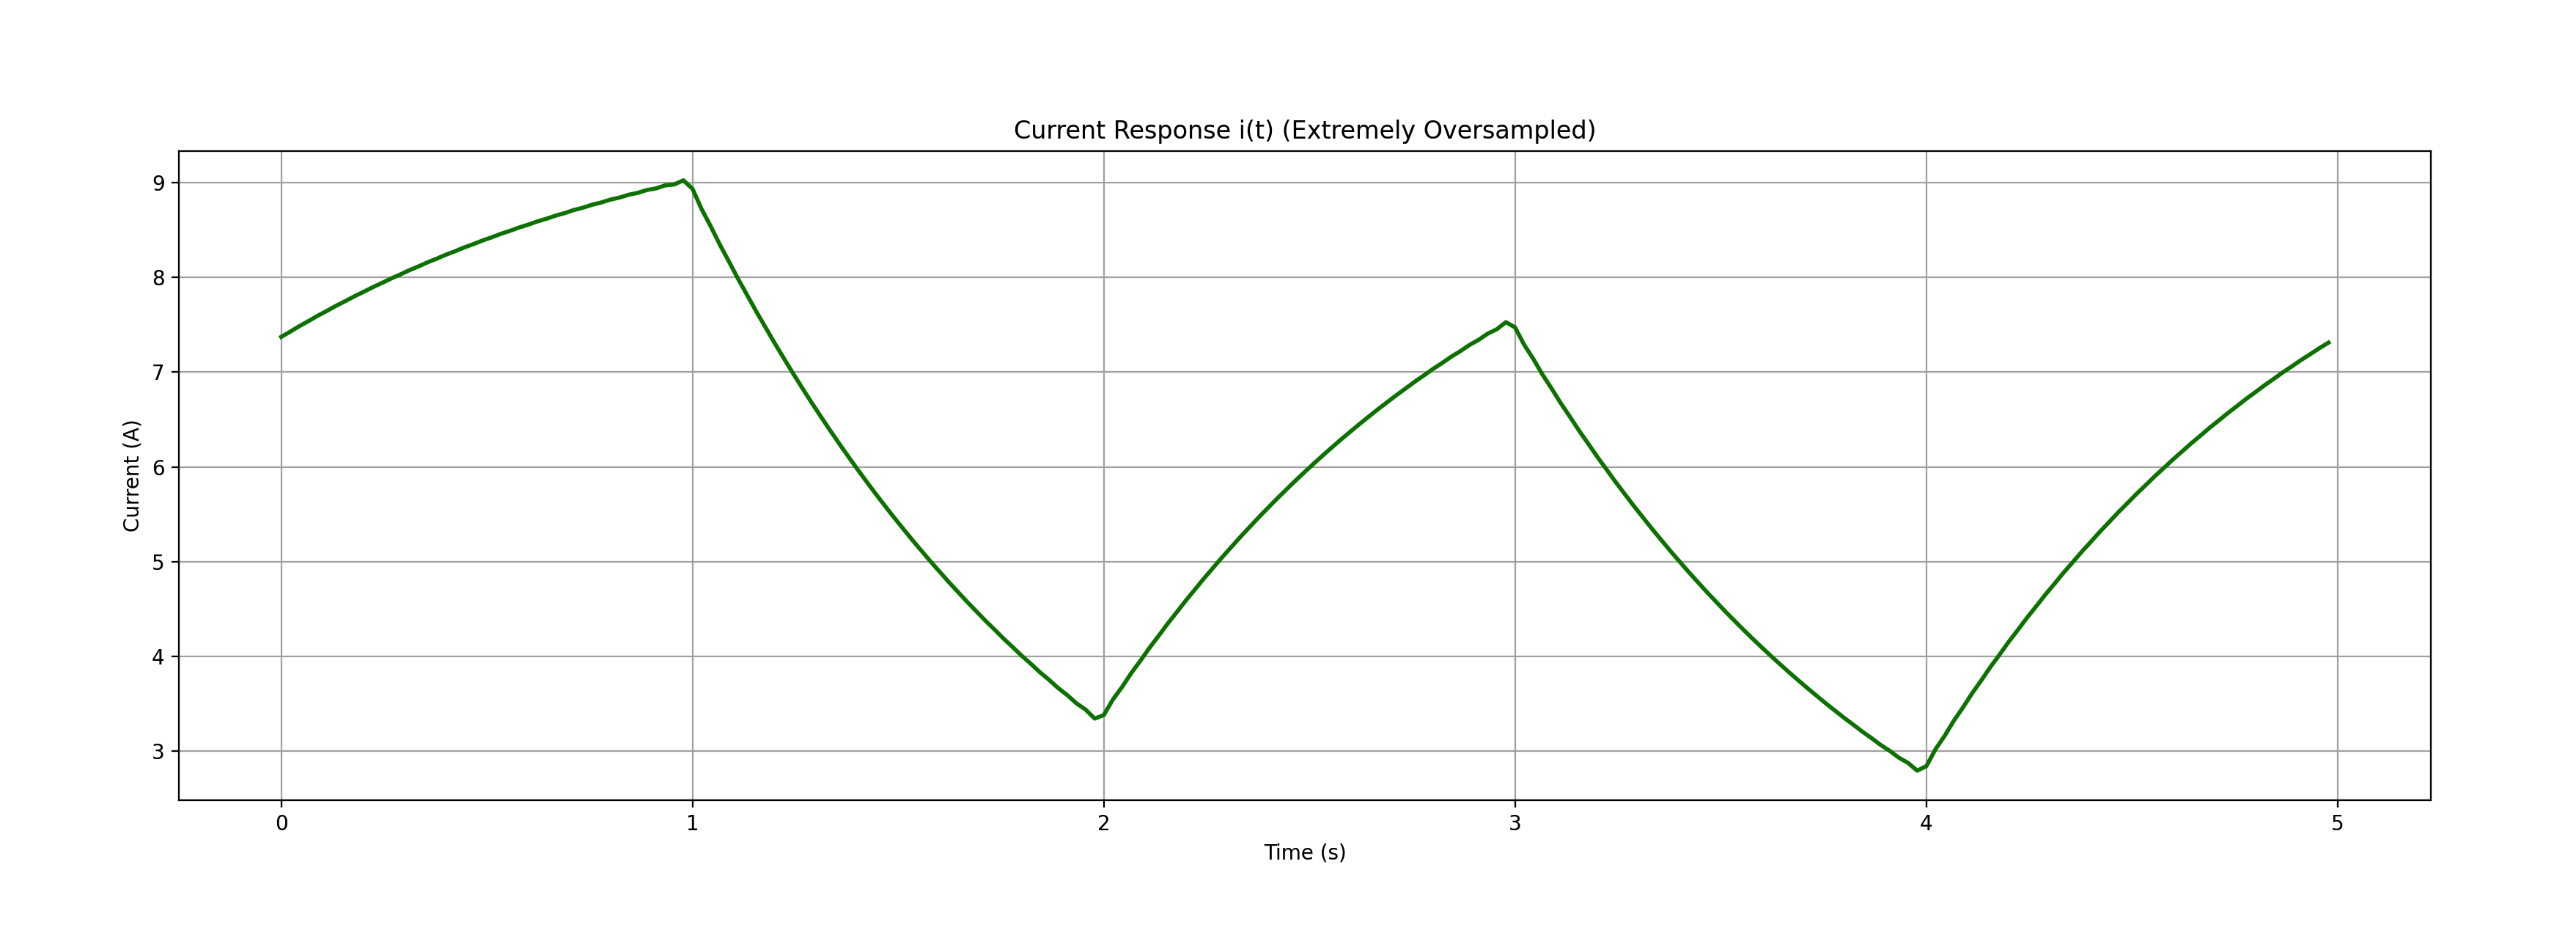
\includegraphics[width=0.6\textwidth]{figs/10_f_ny.png}
    \caption{The current response for  $f_s \gg f_{ny}$   i.e, $(10 f_{ny})$}
    \label{fig:example}
    \begin{itemize}
        \item 	No significant change in the output waveform is observed.
        \item Computation time increases, but results remain nearly the same.
    \end{itemize}
    So it is evident that something about the frequency corresponding to twice the frequency of input wave is special. This special nature is captured by the \textbf{sampling theorem}.

\section{Key Findings: }
\begin{enumerate}
    \item FFT-Based Solution for RL Circuits:
    \begin{itemize}
        \item The FFT method provides an efficient way to analyze linear circuit responses in the frequency domain.
        \item By applying the inverse FFT, we accurately retrieve the time-domain current response.
    \end{itemize}
    \item Nyquist Sampling and Computational Efficiency:
    \begin{itemize}
        \item Sampling at or above the Nyquist rate preserves essential frequency components while minimizing data redundancy.
        \item Increasing the sampling rate beyond a certain threshold does not significantly alter the output current waveform, confirming the sufficiency of Nyquist's criterion.
    \end{itemize}
    \item Effect of Circuit Parameters:
    \begin{itemize}
        \item The RL circuit acts as a low-pass filter, smoothing the square wave input by attenuating higher harmonics.
        \item he response shape is influenced by the resistance R, inductance L, and the duty cycle of the input square wave.
    \end{itemize}
    \item Practical Implications:
    \begin{itemize}
        \item Understanding sampling limitations is crucial for real-world signal processing and embedded systems applications.
        \item The interactive implementation enables real-time visualization of how different parameters affect the circuit's behavior.
    \end{itemize}
\end{enumerate}
% Chapter Template

\chapter{References}

\label{Chapter8} % Change X to a consecutive number; for referencing this chapter elsewhere, use \ref{ChapterX}

\lhead{Chapter 8. \emph{References}}
\begin{enumerate}
    \item 
\href{https://www.ti.com/lit/an/slva477b/slva477b.pdf?ts=1742274977685&ref_url=https%253A%252F%252Fduckduckgo.com%252F}{\textcolor{blue}{This}} sheet inspired the parameter values for efficiency analysis.
\item \href{https://www.ddm.org/DD15/pdf/127.pdf}{\textcolor{blue}{This}} paper should be referred for in depth stability analysis of the Parareal Algorithm.
\item \href{https://ieeexplore.ieee.org/stamp/stamp.jsp?tp=&arnumber=8210523}{This} paper was used for frequency response analysis.
\item Power Electronics by Daniel W. Hart
\end{enumerate}

%----------------------------------------------------------------------------------------
%	THESIS CONTENT - APPENDICES
%----------------------------------------------------------------------------------------

\addtocontents{toc}{\vspace{2em}} % Add a gap in the Contents, for aesthetics

\appendix % Cue to tell LaTeX that the following 'chapters' are Appendices

% Include the appendices of the thesis as separate files from the Appendices folder
% Uncomment the lines as you write the Appendices

%% Appendix Template

\chapter{Local plastic strain measurements} % Main appendix title

\label{AppendixX} % Change X to a consecutive letter; for referencing this appendix elsewhere, use \ref{AppendixX}

\lhead{Appendix A. \emph{Local plastic strain measurements}} % Change X to a consecutive letter; this is for the header on each page - perhaps a shortened title


The plastic deformation in metallic materials is of a heterogeneous nature, with strain distributed non-uniformly at the inter and intragranular levels. In order to evaluate the capabilities of full-field models for predicting the deformation arrangement, experimental techniques are required to measure the spatially resolved deformation formation in microstructures.

\section{Electron Backscatter Diffraction}
\label{Electron Backscatter Diffraction}

Electron Backscatter Diffraction (EBSD) is a technique for measuring crystal orientation using a scanning electron microscope (SEM). A focussed electron beam illuminates a spot on the surface of the sample that is inclined by $70^{\circ}$  to the beam direction. Part of this primary beam is elastically scattered from the crystal lattice. These backscattered electrons diffract through the crystal lattice as they escape the material, producing a spatial electron intensity pattern that indicates the crystal structure and orientation. The diffracted electors emanate spherically from the illuminated point on the sample surface. Since the sample is tilted, a detector can be positioned to collect a portion of the diffraction pattern on a flat plane. The collected Kikuchi pattern (named for a pioneer in electron diffraction) can then be analysed to assess the orientation of the crystal by measuring the position and orientation of bands of constructive interference \cite{maitland2007electron}.

\noindent A crystal orientation map can be collected by rastering the beam across the sample surface, collecting and analysing a Kikuchi pattern at each point. These maps contain information about grain size, grain boundary character, sample texture and alloy phase. EBSD can also be used to assess local deformations \cite{wright2011review}. This is achieved either by direct measurement of elastic strains through cross-correlation of individual Kikuchi patterns \cite{wilkinson2006high,wilkinson2006high,britton2012high} or by quantifying small changes and orientation gradients that are generated by plastic deformation \cite{kamaya2004measurement,kamaya2007local,githinji2013ebsd}.

\subsection{Measures of misorientation}
\label{Measures of misorientation}

Misorientation is the difference between two orientations and can be expressed as the minimum angle of rotation around any axis that transforms one orientation into another. The plastic deformation of a crystal due to dislocation slip induces a rotation of the crystal lattice. In an unrestrained single crystal, this leads to a net rotation of the material. However, in order to ensure that the grains remain compatible with their neighbours in a polycrystal, deformation gradients and differences in active slip system within single grains are required \cite{barbe2001intergranular}. This leads to orientation gradients that develop within the grains. Each active slip system induces rotation around a different axis, and the amount of rotation is proportional to the amount of slip. The changes in orientation are accommodated in the crystal lattice by means of geometrically necessary dislocations (GNDs), which cause a net rotation of the lattice. A GND density can be calculated from the rotation gradients of the lattice \cite{pantleon2008resolving}.

\noindent The measurement parameters for misorientation define between which orientations the misorientation is calculated and how this relates to the crystal rotation. In a class of misorientation parameters, a misorientation between neighbouring spatial points of an EBSD is calculated. This could be a single point in a single direction or, more generally, in a kernel of positions surrounding each point. The average of the misorientation at each point in the kernel results in the kernel-averaged misorientation (KAM) \cite{wright2011review}. The KAM quantifies local fluctuations in orientation. Large values indicate a large local orientation gradient resulting from a change in the active slip system or an abrupt change in slip activity. Examples of KAM maps taken from a plastically deformed sample are shown in figure \ref{fig:Measures of misorientation1}a-b. The EBSD maps are taken at two different EBSD step sizes and show that KAM values are sensitive to the chosen EBSD step size.

\begin{figure}
    \centering
    \includegraphics[scale=1.5]{Pictures/KAM.jpg}
    \caption{Examples of misorientation parameters for the same region of material. a) and b) are KAM calculated for a 3x3 pixel $^{2}$ kernel for EBSD step sizes of $0.2 \mu \mathrm{m}$ and $0.4 \mu \mathrm{m} .$ c) is ROD calculated to each grains average orientation and d) ROD calculated to the point in each grain with minimum KAM. Taken from \cite{wright2011review}.}
    \label{fig:Measures of misorientation1}
\end{figure}

KAM does not indicate gradual changes of orientation relating to gradients of deformation. This can be measured using a second class of parameters, the reference orientation deviation (ROD) \cite{wright2011review}. As the name suggests ROD is the misorientation between each point of a map to a reference orientation.A reference orientation must be defined separately for each grain in the EBSD map, since the misorientation between two grains is generally greater than any gradient in it. Common choices for the reference orientation are the mean orientation of each grain or the point in each grain with the minimum KAM value. Figure \ref{fig:Measures of misorientation1}c-d shows a ROD map for each of these reference orientation choices. Similar gradients can be seen in each map but with different magnitudes of the ROD values, whereby the choice of the reference orientation only changes the zero point of the misorientation. Since ROD measures misorientation relative to a fixed reference, it is not sensitive to step size changes.

\noindent The use of misorientation can indicate intense strain in the grains of a microstructure \cite{kamaya2006quantification}, but cannot identify magnitudes of strains. The distribution of the intragranular plastic strain is also not well predicted due to misorientation compared to local strain measurements from image correlation techniques \cite{kamaya2007local}. The misorientation, however, provides a good measure of the microstructure evolution induced by plastic deformation.
%\input{Appendices/AppendixB}
%\input{Appendices/AppendixC}

\addtocontents{toc}{\vspace{2em}} % Add a gap in the Contents, for aesthetics

\backmatter

%----------------------------------------------------------------------------------------
%	BIBLIOGRAPHY
%----------------------------------------------------------------------------------------

\end{document}  
